% Options for packages loaded elsewhere
\PassOptionsToPackage{unicode}{hyperref}
\PassOptionsToPackage{hyphens}{url}
%
\documentclass[
]{article}
\title{A living review of Interactive Theorem Provers}
\author{Sam Nolan}
\date{29th of September 2021}

\usepackage{amsmath,amssymb}
\usepackage{lmodern}
\usepackage{iftex}
\ifPDFTeX
  \usepackage[T1]{fontenc}
  \usepackage[utf8]{inputenc}
  \usepackage{textcomp} % provide euro and other symbols
\else % if luatex or xetex
  \usepackage{unicode-math}
  \defaultfontfeatures{Scale=MatchLowercase}
  \defaultfontfeatures[\rmfamily]{Ligatures=TeX,Scale=1}
\fi
% Use upquote if available, for straight quotes in verbatim environments
\IfFileExists{upquote.sty}{\usepackage{upquote}}{}
\IfFileExists{microtype.sty}{% use microtype if available
  \usepackage[]{microtype}
  \UseMicrotypeSet[protrusion]{basicmath} % disable protrusion for tt fonts
}{}
\makeatletter
\@ifundefined{KOMAClassName}{% if non-KOMA class
  \IfFileExists{parskip.sty}{%
    \usepackage{parskip}
  }{% else
    \setlength{\parindent}{0pt}
    \setlength{\parskip}{6pt plus 2pt minus 1pt}}
}{% if KOMA class
  \KOMAoptions{parskip=half}}
\makeatother
\usepackage{xcolor}
\IfFileExists{xurl.sty}{\usepackage{xurl}}{} % add URL line breaks if available
\IfFileExists{bookmark.sty}{\usepackage{bookmark}}{\usepackage{hyperref}}
\hypersetup{
  pdftitle={A living review of Interactive Theorem Provers},
  pdfauthor={Sam Nolan},
  hidelinks,
  pdfcreator={LaTeX via pandoc}}
\urlstyle{same} % disable monospaced font for URLs
\usepackage{geometry}
\geometry{a4paper, portrait, margin=3cm}
\usepackage{listings}
\newcommand{\passthrough}[1]{#1}
\lstset{defaultdialect=[5.3]Lua}
\lstset{defaultdialect=[x86masm]Assembler}
\usepackage{longtable,booktabs,array}
\usepackage{calc} % for calculating minipage widths
% Correct order of tables after \paragraph or \subparagraph
\usepackage{etoolbox}
\makeatletter
\patchcmd\longtable{\par}{\if@noskipsec\mbox{}\fi\par}{}{}
\makeatother
% Allow footnotes in longtable head/foot
\IfFileExists{footnotehyper.sty}{\usepackage{footnotehyper}}{\usepackage{footnote}}
\makesavenoteenv{longtable}
\usepackage{graphicx}
\makeatletter
\def\maxwidth{\ifdim\Gin@nat@width>\linewidth\linewidth\else\Gin@nat@width\fi}
\def\maxheight{\ifdim\Gin@nat@height>\textheight\textheight\else\Gin@nat@height\fi}
\makeatother
% Scale images if necessary, so that they will not overflow the page
% margins by default, and it is still possible to overwrite the defaults
% using explicit options in \includegraphics[width, height, ...]{}
\setkeys{Gin}{width=\maxwidth,height=\maxheight,keepaspectratio}
% Set default figure placement to htbp
\makeatletter
\def\fps@figure{htbp}
\makeatother
\setlength{\emergencystretch}{3em} % prevent overfull lines
\providecommand{\tightlist}{%
  \setlength{\itemsep}{0pt}\setlength{\parskip}{0pt}}
\setcounter{secnumdepth}{5}
\newlength{\cslhangindent}
\setlength{\cslhangindent}{1.5em}
\newlength{\csllabelwidth}
\setlength{\csllabelwidth}{3em}
\newlength{\cslentryspacingunit} % times entry-spacing
\setlength{\cslentryspacingunit}{\parskip}
\newenvironment{CSLReferences}[2] % #1 hanging-ident, #2 entry spacing
 {% don't indent paragraphs
  \setlength{\parindent}{0pt}
  % turn on hanging indent if param 1 is 1
  \ifodd #1
  \let\oldpar\par
  \def\par{\hangindent=\cslhangindent\oldpar}
  \fi
  % set entry spacing
  \setlength{\parskip}{#2\cslentryspacingunit}
 }%
 {}
\usepackage{calc}
\newcommand{\CSLBlock}[1]{#1\hfill\break}
\newcommand{\CSLLeftMargin}[1]{\parbox[t]{\csllabelwidth}{#1}}
\newcommand{\CSLRightInline}[1]{\parbox[t]{\linewidth - \csllabelwidth}{#1}\break}
\newcommand{\CSLIndent}[1]{\hspace{\cslhangindent}#1}

\makeatletter
\@ifpackageloaded{subfig}{}{\usepackage{subfig}}
\@ifpackageloaded{caption}{}{\usepackage{caption}}
\captionsetup[subfloat]{margin=0.5em}
\AtBeginDocument{%
\renewcommand*\figurename{Figure}
\renewcommand*\tablename{Table}
}
\AtBeginDocument{%
\renewcommand*\listfigurename{List of Figures}
\renewcommand*\listtablename{List of Tables}
}
\newcounter{pandoccrossref@subfigures@footnote@counter}
\newenvironment{pandoccrossrefsubfigures}{%
\setcounter{pandoccrossref@subfigures@footnote@counter}{0}
\begin{figure}\centering%
\gdef\global@pandoccrossref@subfigures@footnotes{}%
\DeclareRobustCommand{\footnote}[1]{\footnotemark%
\stepcounter{pandoccrossref@subfigures@footnote@counter}%
\ifx\global@pandoccrossref@subfigures@footnotes\empty%
\gdef\global@pandoccrossref@subfigures@footnotes{{##1}}%
\else%
\g@addto@macro\global@pandoccrossref@subfigures@footnotes{, {##1}}%
\fi}}%
{\end{figure}%
\addtocounter{footnote}{-\value{pandoccrossref@subfigures@footnote@counter}}
\@for\f:=\global@pandoccrossref@subfigures@footnotes\do{\stepcounter{footnote}\footnotetext{\f}}%
\gdef\global@pandoccrossref@subfigures@footnotes{}}
\newcommand*\listoflistings\lstlistoflistings
\AtBeginDocument{%
\renewcommand*{\lstlistlistingname}{List of Listings}
}
\makeatother
\ifLuaTeX
  \usepackage{selnolig}  % disable illegal ligatures
\fi
\definecolor{verb_border}{rgb}{0.7,0.7,1}
\definecolor{verb_bg}{rgb}{.95,.96,.97}
\begin{document}
\lstset{  
backgroundcolor=\color{verb_bg},  
frame=single
}
\begin{titlepage}
\begin{figure}[t!]
\centering

\includegraphics[width=5cm]{Images/rmit-logo.png}
\end{figure}

\vspace*{2cm}

\begin{center}
{\large
  A living review of Interactive Theorem Provers\\
	[1cm]
	A thesis submitted in fulfilment of the requirements for the degree of Bachelor of Science.\\
	[2cm]
	Sam Nolan\\
	[0.5cm]
	Computer Science Undergraduate.\\
	[3cm]
	School of Science.\\
	[0.5cm]
	College of Science, Engineering and Health.\\
	[0.5cm]
	RMIT University.\\
	[2cm]
  November 2021\\
}
\end{center}
	
\end{titlepage}

\section*{Declaration}
I certify that except where due acknowledgment has been made, the work
is that of the author alone; the work has not been submitted previously,
in whole or in part, to qualify for any other academic award; the
content of the thesis is the result of work which has been carried out
since the official commencement date of the approved research program;
any editorial work, paid or unpaid, carried out by a third party is
acknowledged; and, ethics procedures and guidelines have been
followed.\\
[1cm]
Signed: Sam Nolan\\
[1cm]
Date: 29th of September 2021\\

\section*{Acknowledgments}
I would like to acknowledge my supervisor Maria Spichkova for her
guidance and high expectations for this project. I would also like to
thank Flora Salim for inspiring me to further invest myself into
research and never stopping in opening doors for me.

\newpage

\begin{abstract}
Interactive Theorem Provers are tools that allow you to prove that
software is correct. However, ITPs are known to be quite difficult to
use and the adoption of ITPs is far from widespread. This thesis
investigates usability issues that exist in literature, and then creates
a living review that that covers progress on different theorem provers,
in order to encourage newcomers to the field and document progress on
the development. This review doubles as a decision tool for deciding
whether an ITP should be used for a project.
\end{abstract}
\newpage

\tableofcontents
\newpage

\hypertarget{introduction}{%
\section{Introduction}\label{introduction}}

This is a thesis about \textbf{Interactive Theorem Provers}, what they
are, how they've been used in the past and whether you should explore
using them in your next project.

An \textbf{Interactive Theorem Prover} (ITP) or \textbf{Proof Assistant}
is a piece of software that helps prove mathematical theorems, or
equivalently, prove correctness properties about software. Some of the
more well known examples of provers include
\href{https://coq.inria.fr/}{Coq} and
\href{https://isabelle.in.tum.de/}{Isabelle}.

An ITP is often used by either a mathematician or an engineer. From the
side of a mathematician, it is possible to prove theorems that the ITP
can prove is correct. This ensures that no errors find themselves into
any proof that's made. ITPs have been used for the QED Manifesto,
POPLMark and proving theorems such as the four colour theorem, and
Mizar's Mathematical Library.

An ITP can however also be used by a software engineer to create
certified software. Certified software is software that's been proven to
operate correctly. This is a very high level of assurance in terms of
quality, and in industry and research today, is often used to ensure
correctness of cryptographic libraries, microcode, kernels and
compilers.

In computer science, often correctness proofs of algorithms (For
example, Dijkstra's algorithm in an undergraduate context) are described
and proved to be correct on pen and paper. The use of an ITP in
analogous to this type of activity.

The task of creating verified software is split into two steps: first
specification and then verification.

During specification, You specify what it is that you would like to
prove, for example, that Dijkstra's algorithm always finds the shortest
path between two nodes in a weighted graph, assuming positive weights.
In this step, you would create a specification for what is Dijkstra's
algorithm, graphs, and shortest paths. Then state that Dijkstra's
algorithm finds the shortest path. This step is far from trivial, and
there exist dedicated specification languages for this such as Z of VDL.

This specification leaves you with a \textbf{proof obligation}. A proof
obligation is a onus on the user to prove that the specification of the
software is correct. Then, during verification, it is then up to the
user to provide to the ITP the reasoning as to why this proposition is
correct. This can be done in several ways, sometimes through the use of
automated software, or manipulating with the proof by pointing and
clicking, or writing down a \textbf{proof script} that describes the
steps made to prove the theorem. Often this involves breaking down one
proof obligation into many other simpler proof obligations that can be
solved individually.

The ITP then checks whether the proof of the proposition is valid,
assisting you along the way in any errors that you make. The user and
the ITP work together until you have specified a proof of the statement
you wish to claim. Once that proof is made, you can be assured that the
system works correctly.

Another way of approaching ITPs is through programming languages. Often
a goal in programming language design is to create languages where you
cannot make a certain class of errors. For instance, Rust is designed to
allow systems level programming that's protected from memory errors, and
Elm is designed to create web programs that do not have runtime errors.
Languages often accomplish this through Type Systems and Functional
Programming. ITPs are languages that have design features that allow you
to go as far as proving the correctness of your software. Almost all
ITPs use Type Systems and Functional Programming to assist in proving
software.

More widespread use of ITPs is valuable as it allows for errors to be
caught much earlier in the development process.

\hypertarget{formal-methods}{%
\subsection{Formal Methods}\label{formal-methods}}

ITPs are not the only way to specify and verify software. They belong to
a class of techniques named \textbf{Formal Methods}.

In essence, formal methods attempts to improve the process that users
can prove the correctness of their software systems. Use of formal
methods can be done without any tools at all, by simply proving
properties by hand, such as the Dijkstra example above.

However, computers and tools have aided people in providing large proofs
for software systems. The tools used in Formal Methods can be roughly
divided into three categories, Model Checkers, Automated Theorem Provers
and Interactive Theorem Provers.

These three techniques are a trade off in three dimensions. You can pick
two but not all three.

\begin{figure}
\hypertarget{fig:formal_methods}{%
\centering
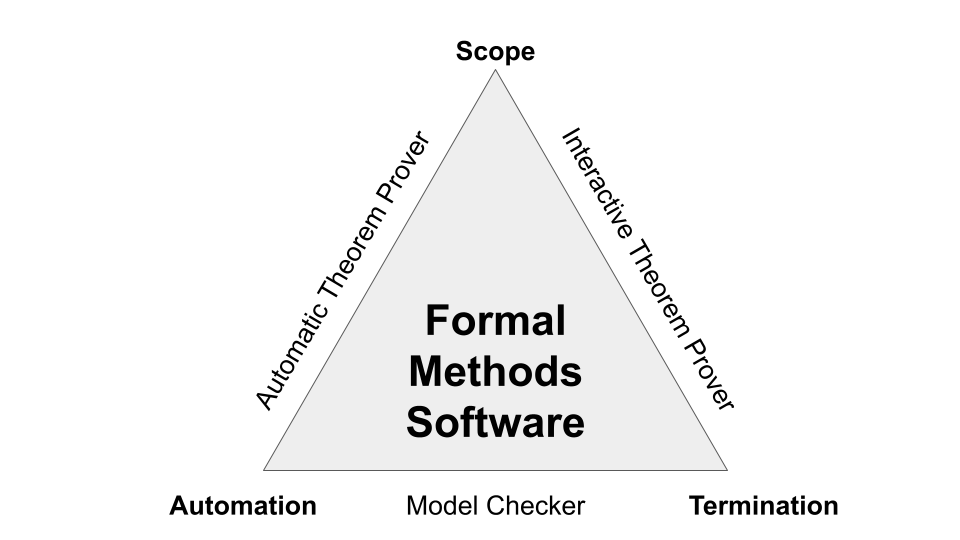
\includegraphics{./Images/formalmethods.png}
\caption{Three categories of Formal Methods}\label{fig:formal_methods}
}
\end{figure}

\textbf{Automation}: Whether finding a proof is fully automated. That
is, the user does not need to specify a proof manually for the
proposition, the system simply attempts to find one automatically.

\textbf{Termination}: Whether the tool terminates in a reasonable amount
of time when attempting to find a proof.

\textbf{Scope}: Whether the system can prove arbitrarily theorems.

\textbf{Model Checkers} are fully automated and terminate in reasonable
time. However, Model checkers can do this by restricting the scope of
the systems that they can prove. They allow for a specification for a
system in a (usually finite) state machine, and can prove properties
about this state machine.

\textbf{Automated Theorem Provers} (ATPs) are fully automated and can
prove arbitrary theorems, however may not terminate in reasonable time.
For larger systems or more complicated theorems, they may run forever
and never identify a proof or disproof for the proposition.

\textbf{Interactive Theorem Provers} terminate in reasonable time and
can prove arbitrary theorems. However, they are not fully automated, and
require the user's input to guide the proof of the theorem.

The distinction between ATPs and ITPs is however not clear cut. ATPs can
often include minor user interaction in order to correct it's path and
find a proof. And ITPs often have automatic features and can even call
external ATPs to discharge proof obligations.

ITPs were chose for this investigation due to their usage in creating
fully verified software such as Coq and SeL4. Although large scale
formalization fully certified software efforts are possible through the
usage of ATPs and Model Checkers, as far as the authors are aware, they
have not been done. Furthermore, ATPs are often used alongside ITPs to
resolve proof obligations automatically, getting the best of both
worlds.

\hypertarget{using-an-itp}{%
\subsection{Using an ITP}\label{using-an-itp}}

Proving properties with an ITP has the flavour of starting with a goal,
and then manipulating that goal into subgoals until you have proven the
proposition.

To demonstrate the usage of an ITP, we will take a look at proving a
theorem in a pseudocode ITP syntax.

Our pseudocode syntax is based on textual theorem provers such as
Isabelle, Coq and HOL. The syntax is simplified to get the basic
concepts of theorem provers across without too many of the confusing
details.

We start with a function:

\[
f(x) = 
  \begin{cases}
    f(x - 1) + x, & x > 0 \\
    0, & x = 0
  \end{cases}
\]

This is the triangle number function. It adds a number to every number
below that number up until 0. For instance,
\(f(5) = 5 + 4 + 3 + 2 + 1 + 0 = 15\).

However, there is a quicker way to calculate the triangle number, and
that is that is that \(f(x) = x(x + 1) / 2\).

This proof is an elementary induction proof. But we shall demonstrate
that this statement is true.

We would like to prove that:

\[ f(x) = x(x + 1)/2 \]

Textual ITPs are in a sense like an interactive programming language.
You write a line of code and then you get an output from this code.

To start with our proof, we write lst.~\ref{lst:proposition} into our
ITP. This statement says that you would like to
\passthrough{\lstinline!Prove!} the statement
\passthrough{\lstinline!forall x, f(x) = x * (x + 1) / 2!}. Prove here
is a keyword that starts the proof. Everything between the
\passthrough{\lstinline!:!} and the \passthrough{\lstinline!.!}
represent the statement you wish to prove.

\begin{lstlisting}[caption={Statement of the proposition you wish to prove}, label=lst:proposition]
Prove: forall x, f(x) = x * (x + 1) / 2.
\end{lstlisting}

After writing this statement, the prover will return to you (often in a
window in the ITP interface, or if it is a command line prover, it will
print it to console) the state lst.~\ref{lst:starting_state}.

The state is separated into two sections, everything above the
\passthrough{\lstinline!---!} is an assumption, that is, what we already
know. We can have multiple assumptions, but in this case, there is none.
Then the statement below the \passthrough{\lstinline!---!} is the
\textbf{goal}. This is the statement that you want to prove. When
starting a proof, whatever statement you want to prove becomes your
first goal, but both the assumptions and the goal will change as you
progress in the proof.

\begin{lstlisting}[caption={Starting state of the prover}, label=lst:starting_state]
---
forall x, f(x) = x * (x + 1) / 2
\end{lstlisting}

It should be noted that during any time during the process, the user may
wish to attempt to prove a goal automatically. Most ITPs have the
ability to automatically prove simple propositions, often by giving the
\passthrough{\lstinline!auto!} command to the prover. If this succeeds,
then the user is done and the proposition is proven. Otherwise, the user
must continue to explore proof options. We will assume that the
statement cannot be proven automatically.

This particular proof is a very common beginners induction proof, so
induction would be a good start to solving this. Entering the pseudocode
in lst.~\ref{lst:induction_tactic} performs induction on the variable x.
To perform induction, we must prove the base case, and then prove the
inductive case. The ITP will get you to prove them one at a time,
starting with the base case. After the command is executed, it will show
the state in lst.~\ref{lst:induction_state}. This means that the theorem
prover is asking you to prove the base case, that is, that the statement
is true when \(x = 0\).

\begin{lstlisting}[caption={Running the induction tactic}, label=lst:induction_tactic]
induction x
\end{lstlisting}

\begin{lstlisting}[caption={State after the induction tactic}, label=lst:induction_state]
---
f(0) = 0 * (0 + 1) / 2
\end{lstlisting}

Notice that the command modifies the state of the ITP. Only commands
that are valid at the time are allowed to be used, ensuring that all
proof steps are valid and construct a correct proof.

The base case is very easy to solve, as simply evaluating the function
on both sides (\(f(0) = 0\) and \(\frac {0 \cdot (0 + 1)}{2} = 0\))
gives 0.

To evaluate this, we use the \passthrough{\lstinline!simplify!} tactic
in lst.~\ref{lst:simplify_tactic}. This tactic attempts to try a list of
rules that the prover guesses will simplify the current statement. In
our pseudocode ITP, this includes evaluating statements between
constants. The result is as we expect and shown in
lst.~\ref{lst:simplify_state}. Indicating that after the simplification,
both sides are equal to each other.

\begin{lstlisting}[caption={Running the simplify tactic}, label=lst:simplify_tactic]
simplify
\end{lstlisting}

\begin{lstlisting}[caption={State after running the simplify tactic}, label=lst:simplify_state]
---
0=0
\end{lstlisting}

Now the goal is to prove that \passthrough{\lstinline!0=0!}. This is
trivially true because equality is reflexive. As of such, we can prove
the current goal by indicating that it's reflexive. This uses the
\passthrough{\lstinline!reflexivity!} tactic in listing
lst.~\ref{lst:reflexivity_tactic}.

Now that we have solved the first goal, the base case, the pseudo-ITP is
now asking us to prove the inductive case
lst.~\ref{lst:reflexivity_state}. It is now our goal to prove the
inductive case. The inductive case now lets us assume that the statement
is true, and that we need to prove that it is the case for x + 1.
Therefore, the statement for proposition for (x + 1) is our goal.

\begin{lstlisting}[caption={Running the reflexivity tactic}, label=lst:reflexivity_tactic]
reflexivity
\end{lstlisting}

\begin{lstlisting}[caption={State after running the reflexivity tactic}, label=lst:reflexivity_state]
f(x) = x * (x + 1) / 2
---
f(x + 1) = (x + 1) * (x + 2) / 2
\end{lstlisting}

The first step would be to evaluate \passthrough{\lstinline!f(x + 1)!}
down by one layer. That is, to replace it with it's definition. This can
be done with the \passthrough{\lstinline!unfold!} command
lst.~\ref{lst:unfold_tactic}. This command replaces a function with it's
definition. This replacement is shown in lst.~\ref{lst:unfold_state}

\begin{lstlisting}[caption={Running the unfold tactic}, label=lst:unfold_tactic]
unfold f
\end{lstlisting}

\begin{lstlisting}[caption={State after running the reflexivity tactic}, label=lst:unfold_state]
f(x) = x * (x + 1) / 2
---
f(x) + (x + 1) = (x + 1) * (x + 2) / 2
\end{lstlisting}

The top and the bottom statements are now identical, they just need
re-arranging for it to be seen. This might involve several commands to
manipulate the state of the equation. We will for the sake of brevity
written these commands in English like code in
lst.~\ref{lst:rearangement_tactics}. The intermediate goals are shown in
lst.~\ref{lst:intermediate_states} to show the progress towards the
desired goal, and the final state is shown in
lst.~\ref{lst:rearangement_state}.

\begin{lstlisting}[caption={Running re-arangement tactics}, label=lst:rearangement_tactics]
expand (x + 1) * (x + 2)
subtract both sides (x + 1)
replace (x + 1) with (2 * (x + 1) / 2)
combine fraction
simplify
factorise (x * x - x)
\end{lstlisting}

\begin{lstlisting}[caption={States after running each command}, label=lst:intermediate_states]
f(x) + (x + 1) = (x^2 + 3x + 2) / 2
f(x) = (x^2 + 3x + 2) / 2 - (x + 1)
f(x) = (x^2 x + 3x + 2) / 2 - ( 2 * (x + 1) / 2)
f(x) = (x^2 + 3x + 2 - 2 * (x + 1)) / 2
f(x) = (x^2 + x) / 2
f(x) = x * (x + 1) / 2
\end{lstlisting}

\begin{lstlisting}[caption={Final state after running each command}, label=lst:rearangement_state]
f(x) = x * (x + 1) / 2
---
f(x) = x * (x + 1) / 2
\end{lstlisting}

Because we know the inductive hypothesis is true, and the goal is
exactly the same as the inductive hypothesis, we can simply indicate
that we have proven the goal. We do this be the
\passthrough{\lstinline!assumption!} command, and then close off the
proof with the \passthrough{\lstinline!QED!} command
lst.~\ref{lst:assumption_tactic}. This then accepts the proof as true
lst.~\ref{lst:assumption_state}.

\begin{lstlisting}[caption={Running the assumption tactic}, label=lst:assumption_tactic]
assumption
QED
\end{lstlisting}

\begin{lstlisting}[caption={State after running the assumption tactic}, label=lst:assumption_state]
Proof accepted
\end{lstlisting}

It should be noted that the commands we wrote out are akin to deduction
rules, however, there is a problem with this approach, and the problem
should become clear once we write down all the commands that you put
into the prover.

\begin{lstlisting}[caption={Final Proof script}, label=lst:final_proof_script]
Prove: f(x) = x * (x - 1) / 2
introduce
induction x
simplify
reflexivity
unfold f
expand (x + 1) * x
subtract both sides x
replace x with (2 * x / 2)
combine fraction
replace ( + x - 2 * x) with ( - x)
factorise (x * x - x)
assumption
QED
\end{lstlisting}

These proof scripts are very difficult to understand statically. Our
understanding of the commands were aided due to our knowledge of the
current state. However, when looking at the script without the context
of the state, they are often very difficult to follow. Especially if the
scripts are more complicated than this one.

This thesis was inspired by the difficulty in reading static proof
scripts. Some provers have already moved to attempt to fix this problem.
For instance, Isabelle's Isar language offers a different way of proving
propositions that embeds more state, and helps the user understand the
proof. It would be therefore valuable to determine what usability issues
have been reported, what has been done to fix them, and whether
solutions from some ITPs could be used to help other provers.

And finally, the secondary motivation of this thesis is to encourage
further use and development of ITPs. So it would be valuable to create a
decision tool that helps a user determine which ITP, if any, should be
used for a particular project.

Hence, the research questions for this thesis are:

RQ1 \emph{What usability issues and solutions have been mentioned in
literature regarding ITPs?}

RQ2 \emph{To what extent to these usability issues exist at the latest
versions of ITPs?}

RQ3 \emph{What, if any, ITP should be used for a specific project?}

\hypertarget{background}{%
\section{Background}\label{background}}

\hypertarget{cognitive-dimensions-of-notation}{%
\subsection{Cognitive Dimensions of
Notation}\label{cognitive-dimensions-of-notation}}

Cognitive Dimensions of Notation is a framework used to evaluate the
effectiveness of
notations~{[}\protect\hyperlink{ref-green_usability_1996}{17}{]}, that
is, ways of writing down information. The notation was originally
proposed by Green as a way of discussing the design trade-offs of visual
programming languages, but has been applied elsewhere for a variety of
notations. These dimensions are not an evaluation framework for
notations, as often increasing one dimension will also change other
dimensions, and different tasks may require different dimensions. For
instance, in textual ITPs, dependencies are not shown between theorems,
and doing so would increase the Diffuseness of the notation, allowing
less to be shown and understood on a single screen. However, debugging
why some theorem might fail given a change in other theorems would aid
from a more diffuse representation showing the hidden dependencies.

Cognitive Dimensions focus mainly on the way that users understand and
work with the meaning of the program. Cognitive Dimensions make an
important distinction between difficulties of understanding and working
with the notation vs difficulties with the actual problem itself.
Because proving theorems is a very cognitively demanding task, that no
matter how perfect the notation will always have an inherit
difficulties. We can only try and improve the notations rather than
making the actual problems easier.

The notation has been adopted as a way of evaluating the usability of
ITPs in Kadoda PhD
Thesis~{[}\protect\hyperlink{ref-kadoda_desirable_1999}{26}{]}. The
interpretation of Cognitive Dimensions in regards to ITPs has been
inspired by their work, but has some notable differences.

The Cognitive Dimensions of Notation are:

\hypertarget{abstraction-gradient}{%
\paragraph{Abstraction Gradient}\label{abstraction-gradient}}

Does the ITP offer ways of abstracting components? Abstraction here
refers to methods, classes and encapsulation. Green classifies notations
as either being abstraction-hating, abstraction-tolerant or
abstraction-hungry. An abstraction-hating ITP would be one that forces
you to work with low level constructs often. An abstraction-tolerant ITP
would be one that gives some methods for abstraction, but still
nevertheless requires constant low level interaction. An
abstraction-hungry ITP would offer many methods of abstraction, that
could even in the end obscure what is actually happening behind the
scenes.

\hypertarget{closeness-of-mapping}{%
\paragraph{Closeness of Mapping}\label{closeness-of-mapping}}

Closeness of Mapping is how similar the notation is to the problem
domain. At some point, a representation of the problem has to be put
into notation suitable for the ITP. The easier this is to do the better
the closeness of mapping, or how close the proof state is represented vs
what the user would expect.

\hypertarget{consistency}{%
\paragraph{Consistency}\label{consistency}}

Once you know the basics of an ITP, how much of the rest can be
inferred? A notation that is not consistent would require constant
lookup of features in the theorem prover. Consistency is particularly
important for learning ITPs. Consistency can become an issue when there
are a large amount of abstractions.

\hypertarget{error-proneness}{%
\paragraph{Error-Proneness}\label{error-proneness}}

Is it easy to make careless mistakes? A common "careless mistake" in
theorem provers is trying to apply a tactic in a textual theorem prover
that is not valid for the current proof state.

\hypertarget{diffuseness}{%
\paragraph{Diffuseness}\label{diffuseness}}

How much does it represent a proof relative to the complexity of the
proposition proven? This is an easier cognitive dimension to measure,
and represents the verbosity of the notation. ITPs with high diffuseness
often have lower abstractions and are easier to understand, but more
difficult to change.

\hypertarget{hard-mental-operations}{%
\paragraph{Hard Mental Operations}\label{hard-mental-operations}}

Are there parts of the notation that require getting out a pencil and
paper to understand what it means? The domain of ITPs by it's very
nature requires Hard Mental Operations, so it's important to separate
the inherit difficulty vs difficulty created by the notation. Hard
Mental Operations may arise out of particularly complicated tactics,
especially since tactics can be composed together. An ITP with a
consistent set of tactics would reduce Hard Mental Operations.

\hypertarget{hidden-dependencies}{%
\paragraph{Hidden Dependencies}\label{hidden-dependencies}}

Are there dependencies in the notation that are not presented? In ITPs
and programming languages, it's usually possible to find what a
function/lemma references, but is difficult to find what
lemmas/functions reference the one we are working in. Furthermore,
automation often uses lemmas in the context without indicating at all
that it is using them. This makes the issue of hidden dependencies even
more difficult. An ITP with low hidden dependencies makes these
dependencies between parts of the program explicit

\hypertarget{perceptual-cues}{%
\paragraph{Perceptual cues}\label{perceptual-cues}}

Does the notation force the user to make decisions before they have the
information they need to make it? Especially for novice users, ITPs need
to allow the user to explore different paths for proving a statement.
This often represents a premature commitment as the user has to commit
to a strategy before evaluating whether that strategy would work. ITPs
that offer undo features and allow postponing making decisions require
less premature commitment.

\hypertarget{premature-commitment}{%
\paragraph{Premature commitment}\label{premature-commitment}}

Does the notation force the user to make decisions before they have the
information they need to make it? Especially for novice users, ITPs need
to allow the user to explore different paths for proving a statement.
This often represents a premature commitment as the user has to commit
to a strategy before evaluating whether that strategy would work. ITPs
that offer undo features and allow postponing making decisions require
less premature commitment.

\hypertarget{progressive-evaluation}{%
\paragraph{Progressive Evaluation}\label{progressive-evaluation}}

Does the system give adequate feedback? Error messages, display of
current proof state and ability to work with incomplete proofs are all
features of progressive evaluation. Getting feedback from the system is
absolutely essential for learning the ITPs.

\hypertarget{role-expressiveness}{%
\paragraph{Role Expressiveness}\label{role-expressiveness}}

Is it easy to identify what the purpose of a component is? Lack of role
expressiveness, particularly within the proofs of textual ITPs, was one
of the main motivations of this study. It is often very difficult on
retrospect to identify how the components of a proof relate to each
other. An ITP with high Role Expressiveness would make it clear how a
lemma or component of a proof contributes to the proof.

\hypertarget{secondary-notation}{%
\paragraph{Secondary Notation}\label{secondary-notation}}

Are there avenues for comments, colours and representation of the code
that helps with comprehension? A Secondary Notation is a way of
representing understanding by not changing the actual meaning of the
notation. ITPs that offer comments, colours and whitespace grouping help
with representing secondary notation.

\hypertarget{viscosity}{%
\paragraph{Viscosity}\label{viscosity}}

Is it easy to make a change in the system? ITPs with low abstraction
make it difficult to make changes. Sometimes a small difference to what
you are wanting to prove requires a disproportionate change of the
proof. ITPs with high viscosity make it difficult to change.

\hypertarget{visibility-and-juxtaposability}{%
\paragraph{Visibility and
Juxtaposability}\label{visibility-and-juxtaposability}}

How easy is to get a particular piece of desired information? How easy
is it to compare part of your proof with proofs elsewhere? Sometimes
critical information is difficult to obtain when creating or
understanding a proof state. A common example is being able to inspect
intermediate proof steps. When a proof relies heavily on automation, it
is sometimes difficult to understand how the automated tactic managed to
get in a particular proof state. Having this information helps
understand the proof and how to move forward. ITPs with low visibility
make it difficult to find such information.

Juxtaposability is showing two parts of the system side by side. This is
important as often a proof might only be a refinement of a previous
proof, and might need to be understood in context.

\hypertarget{methodology}{%
\section{Methodology}\label{methodology}}

To recall our research questions:

RQ1 \emph{What usability issues and solutions have been mentioned in
literature regarding ITPs?}

RQ2 \emph{To what extent to these usability issues exist at the latest
versions of ITPs?}

RQ3 \emph{What, if any, ITP should be used for a specific project?} RQ1
\emph{What usability issues and solutions have been mentioned in
literature regarding ITPs?}

The natural method for answering RQ1 is to perform a systematic
literature review. This literature review intends to identify and
categorize usability issues related to different theorem provers.

Answering RQ2 requires going through the theorem provers and identifying
the issues. However, ITPs are continually in development, and any issue
that arises could be solved at a future date. As of such, we created a
\textbf{living review} to answer this question.

A living review is a literature review of a field that updates
periodically to reflect the current state of the research. These reviews
are often published electronically, such as to a website. The goal of a
living review is to ensure that the review never goes stale, and can be
used as a reference years to come.

This living review is the primary output of this thesis, and although it
has the word ``review'' in it, should not be mistaken for just another
literature review.

It differentiates itself from a normal review by updating automatically
over time, being an interactive software product, and existing as a
decision tool for users.

The creation of this living review will answer RQ3 and RQ2, and provide
descriptions of the current state of the field for ITPs.

\hypertarget{sec:review_methodology}{%
\subsection{Systematic Literature Review
Methodology}\label{sec:review_methodology}}

A preliminary literature review was done in order to survey what
usability problems occurred about theorem provers. This preliminary
review came from a search for ``usability interactive theorem provers"
on the ACM digital library and Google Scholar. The review found several
papers on the topic. We then attempted to construct a query that would
match these papers and also other papers in the field.

Papers were searched for having the title matching the following query:
\passthrough{\lstinline!("Interactive" OR "Deductive") AND ("prover" OR "provers" OR "proving" OR "verifier") AND ("usability" OR "user" OR "users")!}

The justification for using quotes around prover, provers and proving is
that some search engines will return papers with the text "prove" when
looking for "prover". "prove" therefore comes up with many more records
that are unrelated to our topic. "Usability" is also quoted to prevent
searching for "use", which clearly would bring in papers that are
unrelated.

We searched the following databases using this query string:

\begin{itemize}
\tightlist
\item
  Scopus
\item
  DBLP
\item
  Springer Link
\item
  Science Direct
\item
  ACM
\item
  IEEE Xplore
\end{itemize}

From the papers discovered in this way, we went through the abstracts
and discerned whether the paper was relevant to the research question.

Our inclusion criteria for the papers included in the systematic
literature review was the following:

\begin{itemize}
\tightlist
\item
  A peer review published paper AND
\item
  Notes particular usability issues with theorem provers OR
\item
  Offers direct recommendations to the improvement of the usability of
  interactive theorem provers
\end{itemize}

We particularly excluded papers written in languages other than English,
workshops, tutorials, extended abstracts, unpublished and non peer
reviewed papers.

From the papers that were deemed relevant to the research question, we
found papers that cited the papers discovered. That is, we applied
forward snowballing. Semantic scholar was used to perform the forward
snowballing.

We then tried to discover whether these papers were relevant to the
research question, and repeated the process of forward snowballing until
there were no more papers discovered.

We then read the paper to discover:

\begin{itemize}
\tightlist
\item
  A problem and/or solution to usability of interactive theorem provers
\item
  Which theorem prover the issue is relevant to
\item
  Evidence behind issues and proposed solutions
\end{itemize}

The issues were then categorized by Green's cognitive dimensions of
notations~{[}\protect\hyperlink{ref-green_usability_1996}{17}{]}.

\hypertarget{living-review-methodology}{%
\subsection{Living Review Methodology}\label{living-review-methodology}}

The living review has the end goal of determining whether usability
issues still exist, and then further offering a tool to help decision
about ITPs (RQ3).

To do this, the living review is scoped as follows:

\begin{itemize}
\tightlist
\item
  Comparing general properties about ITPs (RQ3)
\item
  Comparing past projects that have been completed by ITPs (RQ3)
\item
  Comparing progress on usability issues about ITPs (RQ2)
\end{itemize}

\hypertarget{general-features-of-about-itps}{%
\subsubsection{General features of about
ITPs}\label{general-features-of-about-itps}}

To compare between different ITPs, general features about them need to
be collected.

We decided to use a 2019 Systematic Literature Reviews on Theorem
Provers as our starting dataset
{[}\protect\hyperlink{ref-nawaz_survey_2019}{32}{]}. This review went
through 27 theorem provers and described the features that each prover
had. This was converted into a dataset and used to compare general
features.

This dataset contained several properties about ITPs, and properties to
compare between them.

The full set of properties are:

\begin{itemize}
\tightlist
\item
  What the ITP is based on
\item
  The logic of the ITP
\item
  The Truth value of the ITP
\item
  Whether it supports Set theory
\item
  Whether it has a library
\item
  What its calculus is
\item
  What's its architecture
\item
  The programming language it's based on
\item
  The User interface
\item
  The Platforms its supported on
\item
  Whether it's scalable
\item
  Multithreaded support
\item
  Whether it has an IDE
\item
  When it was first released.
\item
  Its latest release
\end{itemize}

A lot of these features (such as the logic, truth value etc) require
explanations as to what they refer to. These explanations will be
included within the tool. This allows people unfamiliar to the field to
learn what the components of ITPs are and why they are important.

Some newer ITPs were not included in the dataset, such as Lean, F* and
Idris. These were added manually to the dataset.

The systematic literature review we source our data from however, is
already out of date for the latest release of its provers. As of such,
we have a python script that automatically retrieves whether any newer
versions of a prover have been released by checking GitHub Tags. It gets
the latest tag to be published and adds that as the latest release on
the living review, ensuring that the review doesn't go out of date by
having newer releases.

\hypertarget{comparing-projects-between-itps}{%
\subsubsection{Comparing projects between
ITPs}\label{comparing-projects-between-itps}}

One important thing to consider when making decisions about ITPs to
choose is what past projects have been completed within the ITP. As of
such, we contain a review of different notable projects within the ITP.

Each project will describe:

\begin{itemize}
\tightlist
\item
  The project's name
\item
  The project's scope
\item
  When it was completed
\item
  The ITP used
\end{itemize}

This should help users understand what work has been done with an ITP
before using it. This should help a user decide whether this ITP is
suitable for the task at hand.

\hypertarget{comparing-progress-on-usability-issues-for-itps}{%
\subsubsection{Comparing progress on usability issues for
ITPs}\label{comparing-progress-on-usability-issues-for-itps}}

Finally, depending on the results of the literature review, progress on
different usability issues will be reported in this living review.

How these will be included into the living review will be detailed
later, once those features have been identified.

\hypertarget{literature-review}{%
\section{Literature Review}\label{literature-review}}

The amount of papers found in each section of the review are shown in
tbl.~\ref{tbl:litresults}. This totals to 45 papers found on the topic.
However, 1 paper had to be remove due to not being able to access it,
making 44.

There was a surprisingly small amount of papers caught by query in
comparison to snowballing. This is because many papers that discuss
usability issues about ITPs do not tackle the problem directly (28/38 of
the papers), but rather showcase a feature that has been coded into an
ITP interface. These features do indeed solve a usability problem
implicitly, and represent the bulk of the work on improving interfaces
for ITPs. However, comparatively little research has been done
identifying the issues with ITP interfaces and empirically comparing
these user interface modifications for merit (10/38 of the papers).

\hypertarget{tbl:litresults}{}
\begin{longtable}[]{@{}lll@{}}
\caption{\label{tbl:litresults}Literature review papers}\tabularnewline
\toprule
Round & Found & Relevant \\
\midrule
\endfirsthead
\toprule
Round & Found & Relevant \\
\midrule
\endhead
Query & 45 & 14 \\
Snowball 1 & 121 & 14 \\
Snowball 2 & 191 & 5 \\
Snowball 3 & 99 & 2 \\
Snowball 4 & 44 & 1 \\
Snowball 5 & 4 & 0 \\
\bottomrule
\end{longtable}

When going through papers, it was interesting to find a large amount of
papers proposing user interface models, but not actually identifying the
problems that they solve, nor evaluating their effectiveness. In fact,
out of the 28 papers that showcased user interface improvements, only 2
papers evaluated the their interface improvement to without the
improvement~{[}\protect\hyperlink{ref-berman_development_2014}{12},
\protect\hyperlink{ref-hentschel_empirical_2016}{21}{]}. That there is
not enough empirical studies verifying usability issues has been cited
as an issue that needs to addressed in the
past~{[}\protect\hyperlink{ref-hahnle_deductive_2019}{19}{]}.

The following sections outline usability issues and solutions to those
issues. Tables are included outlining the usability issues mentioned. If
the same problem is mentioned in two papers, it is given two rows.

The theorem prover column refers to the theorem prover the usability
issue was found in. If the problem is a general comment ``General" is
written.''Textual" means a theorem prover that uses proof script to
solve theorems, such as Isabelle/HOL, Coq, Agda. ``Direct Manipulation"
means a theorem prover that uses direct manipulation to solve theorems,
such as KeY.

The discovered column indicates the evidence that that problem exists.
"Suggested" simply means that problem or solution was simply inferred or
has not actually been evaluated as effective. Other values indicate the
type of study that the paper used to observe or evaluate this problem or
solution.

\hypertarget{theorem-provers}{%
\subsection{Theorem Provers}\label{theorem-provers}}

First of all, a brief overview of the theorem provers is in order.

\hypertarget{key}{%
\paragraph{KeY}\label{key}}

KeY is a Direct Manipulation theorem prover, meaning that unlike Textual
theorem provers, does not prove theorems by writing proof scripts, but
instead works by modifying a proof object directly until all proof
obligations have been solved. KeY works by annotating Java programs with
preconditions and postconditions. These conditions are then fed into KeY
as proof obligations. KeY can act as a fully automatic prover, but also
allows the user to attempt to find a proof if the prover fails. KeY has
also formed the basis of KeYmaera and KeYmaera X, which are for proving
properties of hybrid systems.

\hypertarget{hol}{%
\paragraph{HOL}\label{hol}}

HOL is actually a family of theorem provers. Notably HOL4, ProofPower,
HOL Light and HOL Zero. HOL is one of the oldest provers in this list,
and HOL Light is known to be used as a lightweight prover, with a very
easily checkable kernel. HOL provers are textual, and have a simple type
system and use tactics to prove propositions.

\hypertarget{isabelle}{%
\paragraph{Isabelle}\label{isabelle}}

Isabelle (also known as Isabelle/HOL, but for this paper will remain as
Isabelle to prevent confusion) is one of the most popular theorem
provers. The prover has been used for the verification of the SeL4
prover, and exists as the state-of-the-art of ITPs. Isabelle like HOL
has a simple type system and is based of the Logic for Computable
Functions.

\hypertarget{coq}{%
\paragraph{Coq}\label{coq}}

Coq is another popular ITP that also supports a dependent type system.
It's based on the Calculus of (Co)Inductive Constructions, which was
designed specifically for Coq. Coq has been used to prove the four
colour theorem, and create the CompCert certified C compiler.

\hypertarget{matita}{%
\paragraph{Matita}\label{matita}}

Matita is a theorem prover based on Coq's Calculus of (Co)Inductive
Constructions, and was designed to address many of the pain points in
working with Coq. Matita is a much simpler prover that aims to present
the theorem prover as editing a mathematical library. As of such,
Matita's solutions to problems are often pain points in Coq
(mathematical notation, Tinycals etc).

There are a few other provers also in this review, such as iCon, CardiZ
and Dafny. These ITPs are often either coded as proofs of concepts (such
as iCon), or are no longer maintained (in the case of CardiZ or Dafny).
The problems raised by them however, are often relevant for current day
ITPs.

This is by no means a complete list of modern ITPs. Such compilations
have been done~{[}\protect\hyperlink{ref-nawaz_survey_2019}{32}{]}.
These are only the ITPs discussed in the papers found in the review.
There are notable ITPs that are missing from this list that caught us by
surprise, including Agda, Lean and Mizar.

\hypertarget{interaction-paradigms}{%
\subsection{Interaction Paradigms}\label{interaction-paradigms}}

Before moving into the actual problems and solutions found in ITPs, it's
worth giving a short history of the interaction paradigms of ITPs, and
possible developments.

Direct Manipulation ITPs such as KeY work by editing proof objects until
the obligations have been resolved. These provers often have issues with
tedious interactions, and work has even been done add textual elements
to KeY {[}\protect\hyperlink{ref-beckert_interaction_2017}{9}{]}. The
development of interfaces to Direct Manipulation provers often differs
from textual ones.

Textual ITPs such as HOL, Isabelle, Coq and Matita work by writing a
proof script that attempts to prove a proposition. Interacting with
textual ITPs often involves a very simple read-evaluate-print-loop
(REPL) for their interfaces. One very stark example of this is
HOL-Light, which you interact with by opening up the OCaml REPL (a
general purpose ML based functional programming language) and loading
the HOL library. All OCaml is available to you alongside the HOL
library. Although this is rather primitive, modern ITP interfaces such
as Isabelle/jEdit and CoqIDE usually offer only a small layer of
abstraction over a REPL for their own languages.

These interfaces have two main windows, the first has code and the
second has proof state. The code can be evaluated up to a certain point,
and the output from the REPL in terms of proof state are printed in the
second window. The only major difference between this and a standard
REPL is that you can rewind to evaluate up to a previous line. This
simple style of interface has consequences for usability. In particular,
if any error is found either in proof or in syntax, execution stops
until that error is resolved. Further, for larger projects, it can take
a very long time for systems to recompile. It also means that you can
only identify things that have already been identified (it has to be a
single pass). This is particularly an issue when automated tactics
attempt to use lemmas above them to find solutions to theorems (such as
Isabelle). This means that simply changing the order of lemmas in an
Isabelle document, even if they never reference lemmas that are below
them, could cause a lemma that was proven before to become unproven.

Developments in IDEs to allow asynchronous interfaces, reloading only
parts needed and loading proofs out of order have been introduces to fix
this problem. They are called "Prover IDEs", with two examples being
Isabelle/PIDE~{[}\protect\hyperlink{ref-wenzel_asynchronous_2014}{38}{]}
and Coq/PIDE~{[}\protect\hyperlink{ref-barras_asynchronous_2015}{6}{]}.
These hopefully will resolve some of the issues cited above.

Although we have examples of large projects undertaken with ITPs,
optimal interaction paradigms are still up for debate, and several novel
interaction paradigms have surfaced. Including proving theorems and
writing tactics with
diagrams~{[}\protect\hyperlink{ref-grov_tinker_2018}{18},
\protect\hyperlink{ref-lin_understanding_2016}{28},
\protect\hyperlink{ref-shams_accessible_2018}{35}{]}, or providing agent
based
interfaces~{[}\protect\hyperlink{ref-hunter_agent-based_2005}{24}{]}.

We now move into the usability problems and solutions found in ITPs.

\hypertarget{abstraction-gradient-1}{%
\subsection{Abstraction Gradient}\label{abstraction-gradient-1}}

\hypertarget{tbl:abstraction_gradient}{}
\begin{longtable}[]{@{}llll@{}}
\caption{\label{tbl:abstraction_gradient}Abstraction Gradient
Problems}\tabularnewline
\toprule
Theorem prover & Problems & Discovered & citation \\
\midrule
\endfirsthead
\toprule
Theorem prover & Problems & Discovered & citation \\
\midrule
\endhead
KeY & Interaction with low level logic & Focus Groups &
{[}\protect\hyperlink{ref-beckert_usability_2015}{8}{]} \\
Isabelle & Missing Library & Focus Groups &
{[}\protect\hyperlink{ref-beckert_usability_2015}{8}{]} \\
\bottomrule
\end{longtable}

The abstraction gradient dimension concerns itself with the highest and
lowest levels of abstraction that are presented. Are they at the
appropriate level of abstraction?

Issues in this dimension were uncommon. KeY was found to require
interacting on low level logic formulas consistently. Similar issues
with tedious interactions with KeY are mentioned in the viscosity's
section. No solutions were found or suggested to this problem, and it
has not been empirically tested.

Focus Groups found that Isabelle's library lacks the appropriate
mathematical foundations. Interestingly, this is the only issue of this
class and is not mentioned elsewhere, often library issues are more
about managing and searching large libraries, which Matita attempts to
handle, and correct documentation of libraries. This has not been tested
empirically. Other than the implicit solution of providing better
library support for theorem provers, no solution has been provided for
this problem.

\hypertarget{closeness-of-mapping-1}{%
\subsection{Closeness of Mapping}\label{closeness-of-mapping-1}}

\hypertarget{tbl:closeness_of_mapping}{}
\begin{longtable}[]{@{}llll@{}}
\caption{\label{tbl:closeness_of_mapping}Closeness of Mapping
Problems}\tabularnewline
\toprule
Theorem prover & Problems & Discovered & citation \\
\midrule
\endfirsthead
\toprule
Theorem prover & Problems & Discovered & citation \\
\midrule
\endhead
KeY & Unintuitive mapping between formula and program & Focus Groups &
{[}\protect\hyperlink{ref-beckert_usability_2015}{8}{]} \\
CardiZ & Cannot sketch out proofs & Questionnaire &
{[}\protect\hyperlink{ref-kadoda_cognitive_2000}{25}{]} \\
Coq & Cannot use mathematical notation & Survey &
{[}\protect\hyperlink{ref-berman_development_2014}{12}{]} \\
Coq & Cannot use mathematical notation & Suggested &
{[}\protect\hyperlink{ref-asperti_user_2007}{3},
\protect\hyperlink{ref-zacchiroli_user_2007}{41}{]} \\
\bottomrule
\end{longtable}

The dimension of closeness of mapping is whether the interface maps well
to the problem world. For interactive theorem provers, it has to do with
how well the proof state is understood in comparison to the actual
problem.

Focus groups found that because KeY attempts to prove properties through
annotations and java source code, it can sometimes be difficult to see
how this proof state maps to the
program~{[}\protect\hyperlink{ref-beckert_usability_2015}{8}{]}. This
issue is not mentioned in any other source and not tested empirically.
No solutions have been suggested for this.

CardiZ, an ITP that can be used to prove properties of Z specifications,
found that you could not sketch out proofs before an attempt. This is
the only paper on CardiZ, as CardiZ is not a popular prover. No
solutions have been suggested for this.

A common issue that came up with Coq was the inability to use
mathematical notation. Notation issues are problematic in ITPs. One one
hand, theorem provers such as Isabelle and Agda allow using mathematical
notation in their theorems. This helps the user understand the theorem
in a terse syntax. On the other hand, mathematical notation can often be
ambiguous and difficult to type. Isabelle allows using LaTeX~style
commands such as rightarrow to render math notation, whereas Agda allows
Unicode in source files. In order to avoid ambiguity, Coq has no support
for math notation, and in response to this, Matita has LaTeX~style
mathematical notation~{[}\protect\hyperlink{ref-asperti_user_2007}{3},
\protect\hyperlink{ref-zacchiroli_user_2007}{41}{]}. This issue came up
in three different sources.

\hypertarget{consistency-1}{%
\subsection{Consistency}\label{consistency-1}}

\hypertarget{tbl:consistency}{}
\begin{longtable}[]{@{}llll@{}}
\caption{\label{tbl:consistency}Consistency Problems}\tabularnewline
\toprule
Theorem prover & Problems & Discovered & citation \\
\midrule
\endfirsthead
\toprule
Theorem prover & Problems & Discovered & citation \\
\midrule
\endhead
Isabelle & Difficult to know what tactics and lemmas to use & Focus
Groups & {[}\protect\hyperlink{ref-beckert_usability_2015}{8},
\protect\hyperlink{ref-beckert_interaction_2017}{9}{]} \\
HOL & Difficult to know what tactic to apply next & Suggested &
{[}\protect\hyperlink{ref-aitken_interactive_1998}{1}{]} \\
Isabelle & Hard to remember prover specific details & Suggested &
{[}\protect\hyperlink{ref-nagashima_pamper_2018}{31}{]} \\
KeY & Difficult to know what tactic to apply next & Suggested &
{[}\protect\hyperlink{ref-mitsch_keymaera_2017}{30}{]} \\
Isabelle,HOL & Difficult to remember names of theorems & Observational &
{[}\protect\hyperlink{ref-aitken_analysis_2000}{2}{]} \\
Coq & Difficult to find relevant lemmas & Survey &
{[}\protect\hyperlink{ref-berman_development_2014}{12}{]} \\
Coq & Difficult to find arguments for tactics & Observational &
{[}\protect\hyperlink{ref-ringer_replica_2020}{33}{]} \\
Coq & Bad Library, inconsistent naming & Survey &
{[}\protect\hyperlink{ref-berman_development_2014}{12}{]} \\
\bottomrule
\end{longtable}

Consistency is the cognitive dimension of whether, once learning part of
the notation, you are able to infer the rest of the notation.

In textual theorem provers, it is often difficult to remember the name
of the next tactic, theorems or lemmas should be applied in any
situation. This has been bought up in focus
groups~{[}\protect\hyperlink{ref-beckert_usability_2015}{8}{]},
observational
studies~{[}\protect\hyperlink{ref-aitken_analysis_2000}{2}{]},
surveys~{[}\protect\hyperlink{ref-berman_development_2014}{12}{]} and
suggested as a problem from various other sources.

Solutions to this problem often include choosing applicable tactics by
menu~{[}\protect\hyperlink{ref-aitken_interactive_1998}{1},
\protect\hyperlink{ref-aitken_analysis_2000}{2}{]} Which has been
implemented in Coq through Proof
Previews~{[}\protect\hyperlink{ref-berman_development_2014}{12}{]} and
in KeYmaera X~{[}\protect\hyperlink{ref-mitsch_keymaera_2017}{30}{]}.
Machine learning for choosing appropriate recommendations has been
suggested for this
problem~{[}\protect\hyperlink{ref-ringer_replica_2020}{33}{]}, and has
also been implemented through the PaMpeR tool in
Isabelle~{[}\protect\hyperlink{ref-nagashima_pamper_2018}{31}{]}. A
second way of tackling this problem is to improve library searching,
which was
suggested~{[}\protect\hyperlink{ref-aitken_analysis_2000}{2}{]} and is a
focus in
Matita~{[}\protect\hyperlink{ref-tassi_interactive_2008}{37}{]}.
Improving these tools is a promising area for improving the usability of
ITPs

\hypertarget{diffuseness-terseness}{%
\subsection{Diffuseness / terseness}\label{diffuseness-terseness}}

\hypertarget{tbl:diffuseness}{}
\begin{longtable}[]{@{}llll@{}}
\caption{\label{tbl:diffuseness}Diffuseness / Terseness
Problems}\tabularnewline
\toprule
Theorem prover & Problems & Discovered & citation \\
\midrule
\endfirsthead
\toprule
Theorem prover & Problems & Discovered & citation \\
\midrule
\endhead
Isabelle & Bloated Formulas & Focus Groups &
{[}\protect\hyperlink{ref-beckert_usability_2015}{8}{]} \\
Isabelle & Large proofs correspond to large effort & Observational &
{[}\protect\hyperlink{ref-bourke_challenges_2012}{13}{]} \\
\bottomrule
\end{longtable}

Diffuseness is the cognitive dimension of the tersity/verbosity of the
syntax. Bloated formulas were mentioned in Isabelle in Focus Groups, and
projects with more lines of code were strongly correlated with more
effort. No solutions have been suggested to reducing the size of code
bases or formulas.

\hypertarget{error-proneness-1}{%
\subsection{Error Proneness}\label{error-proneness-1}}

\hypertarget{tbl:error_proneness}{}
\begin{longtable}[]{@{}llll@{}}
\caption{\label{tbl:error_proneness}Error Proneness
Problems}\tabularnewline
\toprule
Theorem prover & Problems & Discovered & citation \\
\midrule
\endfirsthead
\toprule
Theorem prover & Problems & Discovered & citation \\
\midrule
\endhead
Isabelle,HOL & Easy to get errors in Object Level Constructions &
Observational & {[}\protect\hyperlink{ref-aitken_analysis_2000}{2}{]} \\
Isabelle,HOL & Incorrect predictions made about tactics & Observational
& {[}\protect\hyperlink{ref-aitken_analysis_2000}{2}{]} \\
Isabelle & Difficult to manage namespace & Suggested &
{[}\protect\hyperlink{ref-bourke_challenges_2012}{13}{]} \\
\bottomrule
\end{longtable}

Error proneness is the cognitive dimension of whether a system allows
its users to make errors.

Observational studies have found that in Isabelle and HOL it is easy to
make errors in syntax. Considering the frequency of syntax errors, this
issue came up surprisingly little other sources. This could be because
syntax errors are relatively easy to fix and also decrease with usage.
It's been suggested that this problem could be solved my improving
feedback in Object Level syntax
input~{[}\protect\hyperlink{ref-aitken_analysis_2000}{2}{]}. A more
interesting solution has been implemented for Coq is a structure editor
based off keyboard
cards~{[}\protect\hyperlink{ref-berman_development_2014}{12}{]}. This
uses rolling chords (like \emph{vi}) keyboard interfaces to interact
with the theorem prover. This means that it is only possible to enter
syntactically valid statements. This current solution only works on a
subset of Coq's syntax. It was found to be slightly quicker than using
dropdown menus.

Sometimes when applying a tactic, an unexpected result would occur,
causing the user to back up and try to understand the current state.
This issue could be solved by Proof
Previews~{[}\protect\hyperlink{ref-berman_development_2014}{12}{]},
which allow you to see a proof state when selecting tactics from a menu
without actually applying the tactic. That way the user can cheaply
explore tactics to continue in the proof.

Finally, for large verification projects such as SeL4, there is an issue
with managing the namespaces of large amounts of theorems and lemmas. No
verification of this problem nor solution has been suggested.

\hypertarget{hard-mental-operations-1}{%
\subsection{Hard mental operations}\label{hard-mental-operations-1}}

\hypertarget{tbl:hard_mental_operations}{}
\begin{longtable}[]{@{}llll@{}}
\caption{\label{tbl:hard_mental_operations}Hard Mental Operations
Problems}\tabularnewline
\toprule
Theorem prover & Problems & Discovered & citation \\
\midrule
\endfirsthead
\toprule
Theorem prover & Problems & Discovered & citation \\
\midrule
\endhead
Coq & Hard to understand proof scripts statically & Suggested &
{[}\protect\hyperlink{ref-zacchiroli_user_2007}{41}{]} \\
General & Difficult to understand tacticals & Suggested &
{[}\protect\hyperlink{ref-grov_tinker_2018}{18},
\protect\hyperlink{ref-lin_understanding_2016}{28}{]} \\
General & Proof scripts can become complicated & Suggested &
{[}\protect\hyperlink{ref-aspinall_towards_2016}{5}{]} \\
\bottomrule
\end{longtable}

The dimension of Hard Mental operations refer to the difficulty in
understanding and using the interface on a syntax level. This type of
issue is common with ITPs, as the actual domain is complicated, so this
is reflected with difficult syntax.

Proofs are hard enough to understand while viewing the dynamic nature of
the proof, investigating proof state bit by bit. They are often near
impossible to understand
statically~{[}\protect\hyperlink{ref-zacchiroli_user_2007}{41}{]}. This
issue has not been investigated empirically, but solutions often involve
changing the syntax around proofs. One notable example of this is Isar
for Isabelle~{[}\protect\hyperlink{ref-wenzel_structured_2006}{40}{]},
which attempts to mirror how a pen and paper proof is structured.

It is often difficult to understand tacticals, and the problem is made
even worse when it is not possible to view the state of a tactical mid
way through interaction. This problem has been suggested in several
sources~{[}\protect\hyperlink{ref-grov_tinker_2018}{18},
\protect\hyperlink{ref-lin_understanding_2016}{28},
\protect\hyperlink{ref-zacchiroli_user_2007}{41}{]} but never
empirically investigated. Solutions to this include representing
tacticals as graphs~{[}\protect\hyperlink{ref-grov_tinker_2018}{18},
\protect\hyperlink{ref-lin_understanding_2016}{28}{]}. This solution has
not been tested with users.

Proof scripts can also get very complicated for larger propositions.
Keeping track of this complexity has been suggested with proof metrics,
which are similar to classic code complexity
metrics~{[}\protect\hyperlink{ref-aspinall_towards_2016}{5}{]}.

\hypertarget{hidden-dependencies-1}{%
\subsection{Hidden dependencies}\label{hidden-dependencies-1}}

\hypertarget{tbl:hidden_dependencies}{}
\begin{longtable}[]{@{}llll@{}}
\caption{\label{tbl:hidden_dependencies}Hidden Dependencies
Problems}\tabularnewline
\toprule
Theorem prover & Problems & Discovered & citation \\
\midrule
\endfirsthead
\toprule
Theorem prover & Problems & Discovered & citation \\
\midrule
\endhead
Isabelle & Hard to see dependencies between proofs & Suggested &
{[}\protect\hyperlink{ref-spichkova_human-centred_2017}{36}{]} \\
KeY & Difficult to patch proofs that have slightly changed & Suggested &
{[}\protect\hyperlink{ref-beckert_evaluating_2012}{10}{]} \\
Isabelle & Hidden automation dependencies & Suggested &
{[}\protect\hyperlink{ref-bourke_challenges_2012}{13}{]} \\
Isabelle & Difficult to patch proofs when dependencies change &
Suggested & {[}\protect\hyperlink{ref-bourke_challenges_2012}{13}{]} \\
Isabelle & Hard to see dependencies between proofs & Suggested &
{[}\protect\hyperlink{ref-aspinall_towards_2016}{5}{]} \\
\bottomrule
\end{longtable}

Hidden dependencies represent dependencies between components that are
not shown explicitly. Hidden dependencies are everywhere in theorem
provers. Like functions in many programming languages, lemmas can
reference the lemmas that they use, but it is difficult to find where a
particular lemma has been used. Automation makes this problem even
worse, where in Isabelle, an automatic tactic will try lemmas that are
above it in the theory. This makes moving lemmas around a theory
document difficult. Moving a lemma around a document, even if all the
other lemmas it is references are above it, may cause it to fail due to
it using a lemma by automation. Monitoring dependencies has been
suggested as part of formal proof metrics. It's been suggested and
implemented within CoqPIE to show these dependencies within the
IDE~{[}\protect\hyperlink{ref-roe_coqpie_2016}{34}{]}. Tools have also
been built to analyse dependencies between Isabelle
proofs~{[}\protect\hyperlink{ref-spichkova_human-centred_2017}{36}{]}.
For automated tactics, Isabelle's sledgehammer offers a unique solution
to showing dependencies. The automatic tactic, after execution, simply
prints a set of manual tactics that were used to prove the theorem into
the document. That way, all the lemmas that were used in the automated
tactic are made
explicit~{[}\protect\hyperlink{ref-bourke_challenges_2012}{13}{]}. None
of these solutions have been empirically tested for validity.

Furthermore, often changing a definition or proof slightly requires
changing the proof in order to match the new definitions. This is a
tedious process.

None of these issues have been tested empirically.

\hypertarget{perceptual-cues-1}{%
\subsection{Perceptual cues}\label{perceptual-cues-1}}

\hypertarget{tbl:perceptual_cues}{}
\begin{longtable}[]{@{}llll@{}}
\caption{\label{tbl:perceptual_cues}Perceptual Cues
Problems}\tabularnewline
\toprule
Theorem prover & Problems & Discovered & citation \\
\midrule
\endfirsthead
\toprule
Theorem prover & Problems & Discovered & citation \\
\midrule
\endhead
HOL & Difficult to understand proof state & Suggested &
{[}\protect\hyperlink{ref-kadoda_cognitive_2000}{25}{]} \\
KeY & Difficult to understand proof state & Suggested &
{[}\protect\hyperlink{ref-hentschel_integrating_2016}{22}{]} \\
General & Difficult to understand proof state & Suggested &
{[}\protect\hyperlink{ref-eastaughffe_support_1998}{14}{]} \\
\bottomrule
\end{longtable}

Perceptual cues is how easy it is to understand what is being
represented. Understanding proof state is an enormous part of theorem
proving. The normal solutions to understanding proof state are to offer
more ways of viewing it, and ensuring easy access to these views. As of
such, solutions are found in the visibility section.

\hypertarget{premature-commitment-1}{%
\subsection{Premature Commitment}\label{premature-commitment-1}}

\begin{longtable}[]{@{}llll@{}}
\caption{Premature Commitment Problems
\{\#tbl:premature\_commitment}\tabularnewline
\toprule
Theorem prover & Problems & Discovered & citation \\
\midrule
\endfirsthead
\toprule
Theorem prover & Problems & Discovered & citation \\
\midrule
\endhead
HOL & Need to redesign model if proof attempt fails & Suggested &
{[}\protect\hyperlink{ref-beckert_usability_2015}{8}{]} \\
Coq & Have to apply tactics before understanding what they do &
Suggested & {[}\protect\hyperlink{ref-berman_development_2014}{12}{]} \\
\bottomrule
\end{longtable}

When an attempt to prove a theorem fails, either one of two things has
happened. First, the proof you are attempting to perform is incorrect,
or the model itself is in error. The model is often in error, and as of
such there is a premature commitment to a model before having a full
understanding. Counterexample generators such as Quick Check and
nitpick~{[}\protect\hyperlink{ref-beckert_usability_2015}{8},
\protect\hyperlink{ref-beckert_interaction_2017}{9}{]} for Isabelle help
prevent the user from trying to prove improvable lemmas by providing the
user with a counterexamples to show why their lemmas can't be true.

Furthermore, tactics often need to be applied to discover what they do.
Typing out this tactic is part of the exploration, and represents
another premature commitment. A cheaper way to explore tactic
applications were trialed with Proof previews in
Coq~{[}\protect\hyperlink{ref-berman_development_2014}{12}{]}. These
proof previews allowed the selection of the next tactic by menu, and
hovering over a tactic previewed it's application in a separate window.
This was found to be helpful with users.

\hypertarget{progressive-evaluation-1}{%
\subsection{Progressive Evaluation}\label{progressive-evaluation-1}}

\hypertarget{tbl:progressive_evaluation}{}
\begin{longtable}[]{@{}llll@{}}
\caption{\label{tbl:progressive_evaluation}Progressive Evaluation
Problems}\tabularnewline
\toprule
Theorem prover & Problems & Discovered & citation \\
\midrule
\endfirsthead
\toprule
Theorem prover & Problems & Discovered & citation \\
\midrule
\endhead
General & Hard to understand why proof state fails & Suggested &
{[}\protect\hyperlink{ref-hentschel_interactive_2016}{23}{]} \\
KeY & Hard to understand why proof state fails & Suggested &
{[}\protect\hyperlink{ref-beckert_usability_2015}{8},
\protect\hyperlink{ref-beckert_interaction_2017}{9},
\protect\hyperlink{ref-beckert_interactive_2015}{11}{]} \\
Dafny & Hard to understand why proof state fails & Suggested &
{[}\protect\hyperlink{ref-grebing_seamless_2020}{15}{]} \\
KeY & Hard to understand why proof state fails & Suggested &
{[}\protect\hyperlink{ref-lin_understanding_2016}{28}{]} \\
General & Hard to understand automated tactics & Suggested &
{[}\protect\hyperlink{ref-mitsch_keymaera_2017}{30}{]} \\
e General & Not enough feedback hinders learning & Suggested &
{[}\protect\hyperlink{ref-mitsch_keymaera_2017}{30}{]} \\
Coq & Lack of background automation & Survey &
{[}\protect\hyperlink{ref-berman_development_2014}{12}{]} \\
General & Lack of background automation & Suggested &
{[}\protect\hyperlink{ref-hunter_agent-based_2005}{24}{]} \\
KeY & Bad feedback hinders learning & Survey &
{[}\protect\hyperlink{ref-beckert_evaluating_2012}{10}{]} \\
Coq & Don't know whether an automated tactic would prove a goal & Survey
& {[}\protect\hyperlink{ref-berman_development_2014}{12}{]} \\
Isabelle & Non reactive interfaces & Suggested &
{[}\protect\hyperlink{ref-beckert_usability_2015}{8}{]} \\
Isabelle & Hard to understand errors from bad inferences of types &
Suggested & {[}\protect\hyperlink{ref-beckert_usability_2015}{8}{]} \\
Isabelle & Performance of automatic strategy & Suggested &
{[}\protect\hyperlink{ref-beckert_usability_2015}{8}{]} \\
Isabelle,KeY & Difficult to understand automated strategy & Suggested &
{[}\protect\hyperlink{ref-beckert_usability_2015}{8}{]} \\
\bottomrule
\end{longtable}

Progressive evaluation is the dimension of getting appropriate feedback
from the system.

Not understanding why proof attempts fails in a widely cited example of
this. This becomes especially true when automation is added to the mix.
Insight to the operation of automated tactics is missing in many ITPs.
This has been suggested to be one of the largest issues with the
usability of ITPs in Focus
Groups~{[}\protect\hyperlink{ref-beckert_usability_2015}{8}{]}. Although
there is little empirical evidence of this issue, the fact that it is so
widely cited indicates importance. Solutions to this issue often resolve
around providing better visibility, and are covered there.

Other issues include that systems with low feedback make it difficult to
teach using ITPs, and that ITPs do not effectively use background
processing to provide the user with feedback. One way of improving
feedback is using a cache of proof
state~{[}\protect\hyperlink{ref-berman_development_2014}{12},
\protect\hyperlink{ref-bourke_challenges_2012}{13}{]}. Another more
novel way is to provide an agent based interaction
model~{[}\protect\hyperlink{ref-hunter_agent-based_2005}{24}{]}, where
the user interfaces have a "Personal assistant", who then negotiates
with proof agents to help solve a particular proof. This makes best use
of background processing while the user is trying to solve a problem.
Neither of these have been tested with users.

Finally, it was mentioned in a survey of Coq users that it would be nice
to know in advance whether an automated tactic could prove a goal. This
would prevent further unnecessary work.

\hypertarget{secondary-notation-1}{%
\subsection{Secondary Notation}\label{secondary-notation-1}}

Secondary notation is the realm of comments, documentation, and even use
of visual placement to convey meaning. Problems due to lack of secondary
notation are usually simply because of missing features, and are
therefore more naturally discussed as solutions.

\hypertarget{tbl:secondary_notation}{}
\begin{longtable}[]{@{}llll@{}}
\caption{\label{tbl:secondary_notation}Secondary Notation
Solutions}\tabularnewline
\toprule
Theorem prover & Intervention & Discovered & citation \\
\midrule
\endfirsthead
\toprule
Theorem prover & Intervention & Discovered & citation \\
\midrule
\endhead
HOL & Allow notes in tree contexts & Suggested &
{[}\protect\hyperlink{ref-aitken_interactive_1998}{1}{]} \\
Isabelle,HOL & Allow adding notes to proof context & Suggested &
{[}\protect\hyperlink{ref-beckert_evaluating_2012}{10}{]} \\
Isabelle & Add document orientated features & Suggested &
{[}\protect\hyperlink{ref-wenzel_isabelle_2011}{39}{]} \\
Isabelle & Gravity for automated lemma placement & Suggested &
{[}\protect\hyperlink{ref-bourke_challenges_2012}{13}{]} \\
Isabelle & Deprecation tags & Suggested &
{[}\protect\hyperlink{ref-bourke_challenges_2012}{13}{]} \\
Coq & Doc comments & Survey &
{[}\protect\hyperlink{ref-berman_development_2014}{12}{]} \\
HOL/CardiZ & Colour and low secondary notation & Survey &
{[}\protect\hyperlink{ref-kadoda_cognitive_2000}{25}{]} \\
Coq & Lack of good tutorials and documentation & Survey &
{[}\protect\hyperlink{ref-berman_development_2014}{12}{]} \\
KeY & Poor documentation & Suggested &
{[}\protect\hyperlink{ref-beckert_evaluating_2012}{10}{]} \\
Isabelle & Better libraries and documentation & Suggested &
{[}\protect\hyperlink{ref-berman_development_2014}{12}{]} \\
\bottomrule
\end{longtable}

One improvement on secondary notations is the ability to note and label
parts of proof context. Usually, proof context is boxed off and cannot
be documented other than basic comments. Interestingly, although this
feature is cited multiple times. It remains, to the best of my
knowledge, unimplemented, and as with the rest of the solutions in this
category, untested.

Document oriented proof organization tries to make each theory readable
both to a human and to a computer, and involves allowing linking to
external theories, websites, diagrams and other features all in the
prover editor. This is commonly done with web interfaces controlled by
ITP code. This method has not been investigated as being beneficial, but
Matita itself was built to support this style of interaction.

Features such as deprecation tags, doc comments and automatic naming of
lemmas frequently showed up. These indicate that it is important for the
user to break out and write hints to help themselves and others navigate
their code. These have been implemented in some provers, but again, have
not been tested.

Finally, a very common issue with ITPs is the lack of tutorials and
documentation, particularly around library functionality. This is
remarkably important, regardless of what the prover is.

\hypertarget{viscosity-1}{%
\subsection{Viscosity}\label{viscosity-1}}

\hypertarget{tbl:viscosity}{}
\begin{longtable}[]{@{}llll@{}}
\caption{\label{tbl:viscosity}Viscosity Problems}\tabularnewline
\toprule
Theorem prover & Problems & Discovered & citation \\
\midrule
\endfirsthead
\toprule
Theorem prover & Problems & Discovered & citation \\
\midrule
\endhead
Isabelle & Messy Downwards compatibility & Focus Groups &
{[}\protect\hyperlink{ref-beckert_usability_2015}{8}{]} \\
Isabelle & No support for proof refactoring & Focus Groups &
{[}\protect\hyperlink{ref-beckert_usability_2015}{8}{]} \\
Direct Manipulation & Tedious Interactions & Suggested &
{[}\protect\hyperlink{ref-beckert_usability_2015}{8},
\protect\hyperlink{ref-grebing_usability_2020}{16}{]} \\
General & Hard to make effective use of large library & Suggested &
{[}\protect\hyperlink{ref-asperti_considerations_2010}{4},
\protect\hyperlink{ref-tassi_interactive_2008}{37}{]} \\
Isabelle & Tacticals difficult to write & Suggested &
{[}\protect\hyperlink{ref-becker_lassie_2021}{7}{]} \\
Coq & Have to update proofs once definition changes & Suggested &
{[}\protect\hyperlink{ref-ringer_replica_2020}{33}{]} \\
Coq & Proof renaming and refactoring is tedious & Suggested &
{[}\protect\hyperlink{ref-ringer_replica_2020}{33}{]} \\
Coq & Large proof scripts require too long to recompile & Suggested &
{[}\protect\hyperlink{ref-barras_asynchronous_2015}{6}{]} \\
Isabelle & Large proof scripts require too long to recompile & Suggested
& {[}\protect\hyperlink{ref-wenzel_asynchronous_2014}{38}{]} \\
Coq & Difficult to select terms & Survey &
{[}\protect\hyperlink{ref-berman_development_2014}{12}{]} \\
Coq & Unnecessary re-running of proofs & Survey &
{[}\protect\hyperlink{ref-berman_development_2014}{12}{]} \\
Coq & Slow for large proofs & Suggested &
{[}\protect\hyperlink{ref-roe_coqpie_2016}{34}{]} \\
Coq & Change in lemma requires change in proof & Suggested &
{[}\protect\hyperlink{ref-roe_coqpie_2016}{34}{]} \\
KeY & Bad change management & Suggested &
{[}\protect\hyperlink{ref-beckert_evaluating_2012}{10}{]} \\
KeY & Bad Automated proof performance & Suggested &
{[}\protect\hyperlink{ref-beckert_evaluating_2012}{10}{]} \\
KeY & Hard to decompose proof & Suggested &
{[}\protect\hyperlink{ref-beckert_interactive_2015}{11}{]} \\
\bottomrule
\end{longtable}

Viscosity is the cognitive dimension of the ease of changing the state
of the programs.

One source of viscosity is simply performance. As automatic strategies
get more complicated, their performance becomes important for them to be
useful to the user. This has been suggested by focus groups and in
surveys. This becomes a particularly difficult problem especially for
larger systems. Attempts to improve performance have been done by
asynchronously loading only required parts of the proof in
Coq~{[}\protect\hyperlink{ref-barras_asynchronous_2015}{6}{]} and
Isabelle~{[}\protect\hyperlink{ref-wenzel_asynchronous_2014}{38}{]}.
Improvements to performance of automatic strategies will always be an
improvement~{[}\protect\hyperlink{ref-bourke_challenges_2012}{13}{]},
including making better use of the
library~{[}\protect\hyperlink{ref-asperti_considerations_2010}{4},
\protect\hyperlink{ref-tassi_interactive_2008}{37}{]}.

A second source is the need to make trivial interactions when making
small changes. For instance, the renaming of a lemma might mean you need
to go through several files to find where to change the identifier.
Messy downwards compatibility, changing definitions, and lack of
refactoring are all examples of this. These are usually addressed by
refactoring tools that have been suggested as
necessary~{[}\protect\hyperlink{ref-bourke_challenges_2012}{13},
\protect\hyperlink{ref-ringer_replica_2020}{33}{]} and implemented in
some IDEs such as
CoqPIE~{[}\protect\hyperlink{ref-roe_coqpie_2016}{34}{]}. These
solutions have not been tested with users.

The third is simply interactions that are tedious and error prone. This
is more common in direct manipulation theorem provers such as KeY. No
solutions have been suggested for this problem.

Finally, the fourth source of viscosity is clunky syntax, such as the
need to explain selections to the theorem prover. Selections are a
common issue where you need to describe the part of the goal that you
want to rewrite. This part might be complicated, but has to be
represented textually. This has served as a challenge for ITP designers.
Selections using patterns has been implemented in
Matita~{[}\protect\hyperlink{ref-asperti_user_2007}{3},
\protect\hyperlink{ref-zacchiroli_user_2007}{41}{]} to address this pain
point.

\hypertarget{visibility}{%
\subsection{Visibility}\label{visibility}}

\hypertarget{tbl:visibility}{}
\begin{longtable}[]{@{}llll@{}}
\caption{\label{tbl:visibility}Visibility Problems}\tabularnewline
\toprule
Theorem prover & Problems & Discovered & citation \\
\midrule
\endfirsthead
\toprule
Theorem prover & Problems & Discovered & citation \\
\midrule
\endhead
KeY & Proof tree too detailed & Focus Groups &
{[}\protect\hyperlink{ref-beckert_usability_2015}{8}{]} \\
Textual & Limited insight to automated tactics & Suggested &
{[}\protect\hyperlink{ref-grebing_usability_2020}{16}{]} \\
HOL & Hard to understand proof tree & Suggested &
{[}\protect\hyperlink{ref-aitken_interactive_1998}{1}{]} \\
HOL & Allow showing and hiding of proof contexts & Suggested &
{[}\protect\hyperlink{ref-aitken_interactive_1998}{1}{]} \\
Coq & Cannot see intermediate proof states & Suggested &
{[}\protect\hyperlink{ref-zacchiroli_user_2007}{41}{]} \\
Coq & Difficult to see structure of proof tree & Suggested &
{[}\protect\hyperlink{ref-berman_development_2014}{12}{]} \\
Coq & Cannot see the relation between subgoals & Survey &
{[}\protect\hyperlink{ref-berman_development_2014}{12}{]} \\
Coq & Cannot quickly see type or simplification of term & Survey &
{[}\protect\hyperlink{ref-berman_development_2014}{12}{]} \\
KeY & Bad presentation of incomplete proofs & Suggested &
{[}\protect\hyperlink{ref-beckert_evaluating_2012}{10}{]} \\
\bottomrule
\end{longtable}

Visibility was a commonly cited issue with interactive theorem provers.

The cognitive dimension of visibility has to do with being able to how
information can be identified and accessible to the user. For the case
of interactive theorem provers, there were cases where theorem provers
show too much or too little information.

Direct manipulation theorem provers such as KeY were found to show too
much information in the proof tree, which overwhelms the user trying to
work out why a proof attempt has failed. The simplest solution to this
is to only show information
needed~{[}\protect\hyperlink{ref-eastaughffe_support_1998}{14}{]} and
allow the opening and closing of
views~{[}\protect\hyperlink{ref-aitken_interactive_1998}{1}{]}. However,
some IDEs (such as CoqIDE) come without a proof tree. These have been
considered
helpful~{[}\protect\hyperlink{ref-aitken_interactive_1998}{1},
\protect\hyperlink{ref-berman_development_2014}{12}{]} and have been
implemented with
Traf~{[}\protect\hyperlink{ref-kawabata_traf_2018}{27}{]}

In contrast, it's also been claimed that there is a lack of visibility
of the proof state, particularly intermediate proof states within
textual theorem provers. The lack of visibility is often to do with
intermediate proof states. An intermediate proof state is the state that
a proof is in before the full completion of a tactic, and can be used to
determine how a tactic got to a particular proof state. Understanding
these intermediate proof states is important in understanding the
process of automatic theorem provers and the current state. Viewing
intermediate proof states is not possible with Isabelle/HOL or Coq. In
fact, it is not even possible to investigate the inside of tacticals
making it even more difficult to understand intuitively a proof. The
tactical problem has been resolved by only using a subset of tacticals
with Matita's Tinycals~{[}\protect\hyperlink{ref-asperti_user_2007}{3},
\protect\hyperlink{ref-zacchiroli_user_2007}{41}{]}. KeYmaera X also
offers traceability with automatic tactics, allowing insight to the
operations they
performed~{[}\protect\hyperlink{ref-mitsch_keymaera_2017}{30}{]}.

In one of the only empirical tests of two different user interfaces, an
interface akin to a symbolic debugger is compared against the standard
interface of
KeY~{[}\protect\hyperlink{ref-hentschel_empirical_2016}{21}--\protect\hyperlink{ref-hentschel_interactive_2016}{23}{]}.
The symbol debugger was found to be easier to use. The interfaces are
very different, and it could be for a variety of reasons. One such
reason is that the interface of a symbolic debugger maps better onto the
context of source code, and offers visibility of that connection.
Offering different ways of viewing and interacting with proof state has
been suggested as a way forward in the usability of
ITPs~{[}\protect\hyperlink{ref-eastaughffe_support_1998}{14},
\protect\hyperlink{ref-grebing_seamless_2020}{15}{]}.

Diagrammatic representations of proof is an alternative way of proving
theorems, as demonstrated with
iCon~{[}\protect\hyperlink{ref-shams_accessible_2018}{35}{]} and Proof
Transitions in
CoqEdit~{[}\protect\hyperlink{ref-berman_development_2014}{12}{]}. This
has not been tested empirically against other ITPs

\hypertarget{analysis}{%
\subsection{Analysis}\label{analysis}}

Many problems were identified. A summary of the problem is tabulated in
fig.~\ref{fig:usability_issues}.

\begin{figure}
\hypertarget{fig:usability_issues}{%
\centering
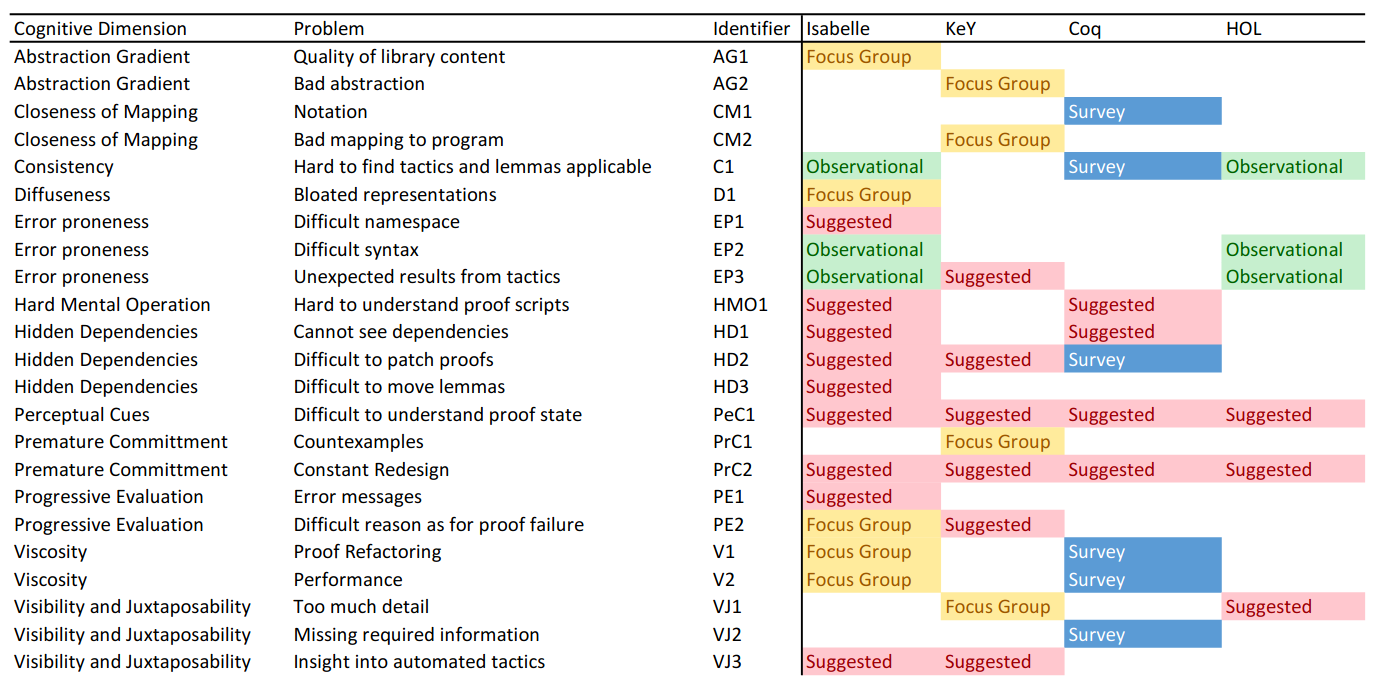
\includegraphics{./Images/MyProblem.png}
\caption{Identified Usability Issues}\label{fig:usability_issues}
}
\end{figure}

This analysis finds that although many issues were identified, there is
very little empirical research on these problems. This is probably due
to the difficulty in recruiting expert participants to these studies,
and the small size of the field.

An empirical analysis of all of these problems is well and truly outside
the scope of this thesis. The task at hand is to now select problems
that can be addressed.

The first thing to consider is that we are creating a living review.
Many of the usability issues that arose have a strong human component.
For instance, ``Hard to predict the results of tactics'' would be very
difficult to evaluate without performing a usability test. If we were to
include a measure within the living review that required the conducting
of a usability test, the usability test would need to be run on a
periodic basis to keep it up to date with the current state of
technology. This is highly undesirable, as such a project would be
extremely time consuming and expensive, and would require a time and
money investment for years after this thesis is published.

To address this, we restrict this thesis to usability issues that can be
determined to exist without the highly expensive intervention of a user.
This leaves the following options:

\begin{itemize}
\tightlist
\item
  Quality of Library
\item
  Notation support
\item
  Counterexamples
\item
  Performance
\end{itemize}

We considered all these issues beside performance to be within the scope
of our living review.

\hypertarget{scope-of-library}{%
\subsubsection{Scope of Library}\label{scope-of-library}}

In a focus group\textasciitilde{}\cite{beckert_usability_2015}, it was
found that Isabelle/HOL was missing important mathematical foundations
in their library.

We decided to evaluate whether these problems still exist by evaluating
the scope of library support of ITPs. This library support also includes
the package systems. For instance, Isabelle has both a standard library
and it's Archive of Formal Proofs. This archive contains mathematics
that is submitted by Isabelle users, and was also included while
evaluating the scope of the ITPs.

First, we collected modules within the ITP libraries, and then we sorted
these packages into the Mathematical Subject Classification 2020
(MSC2020). MSC2020 is a classification of mathematics often used to
classify math papers.

This will allow for a comparison of the scope of ITP libraries

\hypertarget{results}{%
\section{Results}\label{results}}

The result of the living review was the following tool:

\hypertarget{itps}{}

https://samnolan.me/thesis

The living review classified 17 different ITPs, and 11 different
libraries from those ITPs, totalling about 300 math packages.

The ITPs covered in this review were:

\begin{itemize}
\tightlist
\item
  ACL2
\item
  Isabelle
\item
  Atelier B
\item
  Metamath
\item
  Twelf
\item
  Agda
\item
  Mizar
\item
  HOL
\item
  RedPRL
\item
  Coq
\item
  PVS
\item
  Yarrow
\item
  Watson
\item
  JAPE
\item
  LEO-II
\item
  Getfol
\item
  Z/EVES
\end{itemize}

The libraries covered in this review were:

\begin{itemize}
\tightlist
\item
  ACL2's Community Books
\item
  Isabelle's Standard Library
\item
  Isabelle's Archive of Formal Proofs
\item
  Metamath's Proof Library
\item
  Agda's ``standard library''
\item
  Agda's community libraries
\item
  Mizar's Mathematical Library
\item
  HOL's standard library
\item
  Coq's Standard Library
\item
  Coq's Package Ecosystem
\item
  PVS's NASA Library
\end{itemize}

It should be noted that Although Twelf and RedPRL have library support
and a standard library, they were excluded from this review as they are
much too small to be useful for a mathematician, and only include basic
building blocks for building programs in the respective languages.

\hypertarget{math-classifications}{%
\subsection{Math Classifications}\label{math-classifications}}

As of October 2021, after classifying all the packages, it was found
that Isabelle had one of the largest package collections. This seems to
contradict the finding that Isabelle was missing mathematical
foundations, at least relatively speaking.

\begin{figure}
\hypertarget{fig:math_classifications}{%
\centering
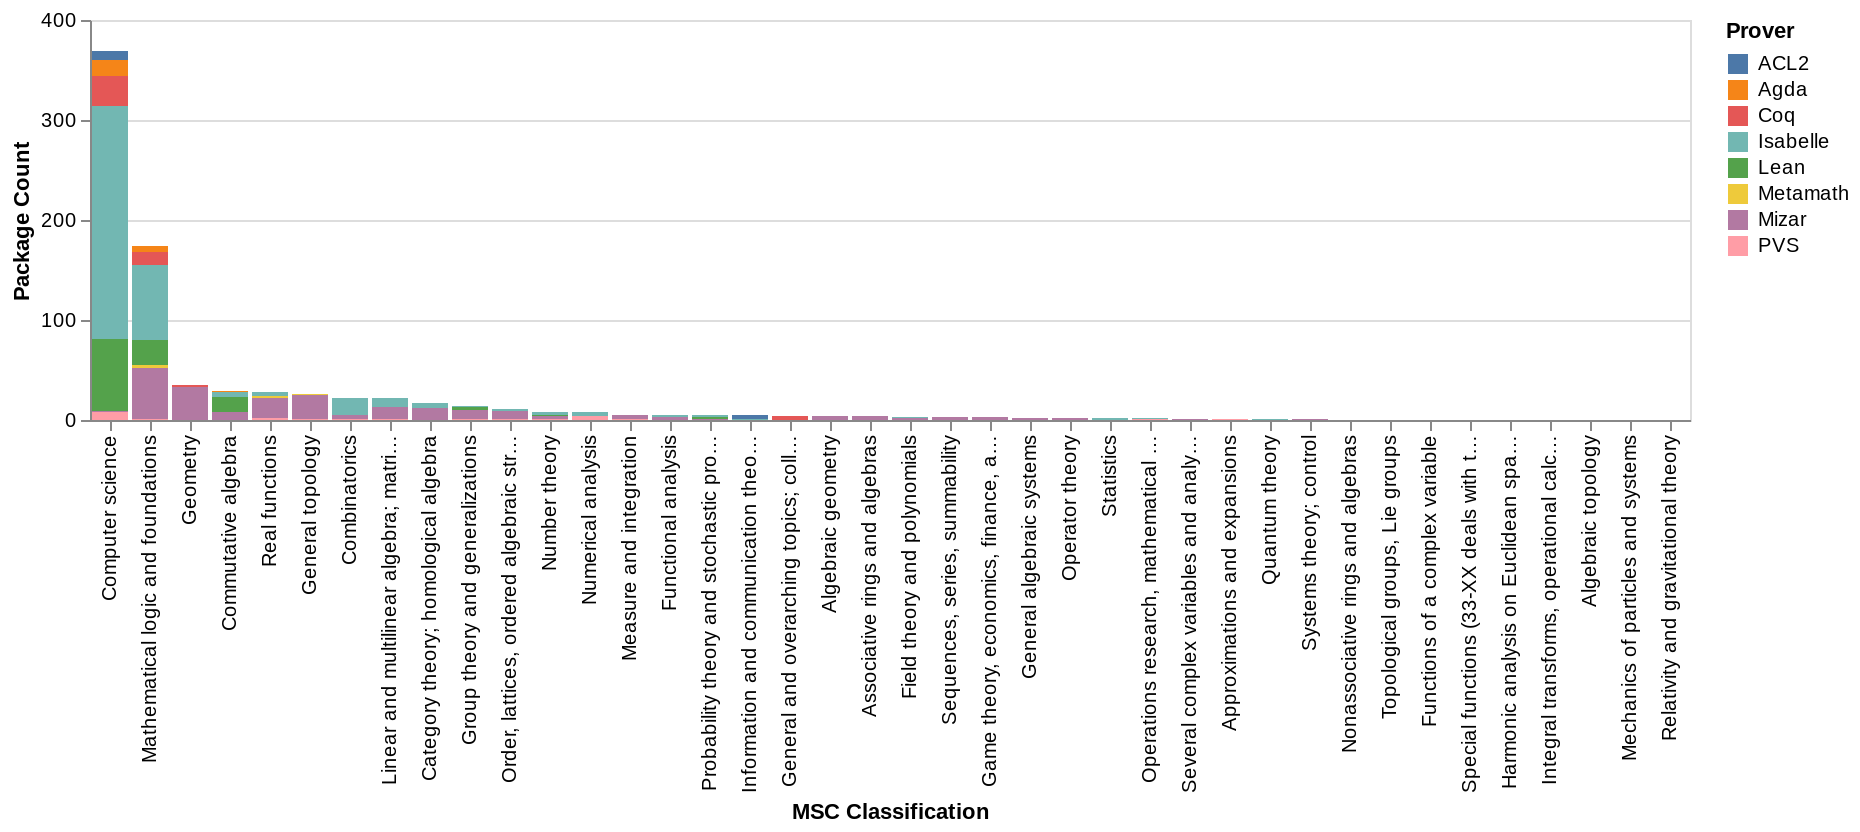
\includegraphics{./Images/MathClassification.png}
\caption{Math Package classifications, as of October
2021}\label{fig:math_classifications}
}
\end{figure}

fig.~\ref{fig:math_classifications} shows verified packages as reported
by the utility on October 2021. It shows that of all packages, most
contributions go to Computer Science (68-XX) and Mathematical Logic and
Foundations (03-XX). This indicates that ITPs have a larger audience
among computer scientists rather than mathematicians. Further work could
go into developing resources for other areas.

Behind that, combinatorics has the largest number of packages verified
in this category, with most algorithms being under graph theory. This
also indicates a tendency for computer science related works due to
graph theory's prominence in computing problems.

The rest of the categories only had a few packages in each, indicating
there is still much to be desired for in other areas of mathematics for
ITPs. However, this result does give the opportunity for mathematicians
to find the few similar efforts that have been done in their field of
interest.

As for provers, Isabelle has the largest mathematical library, followed
by Coq and then ACL2. This indicates that mathematical users should
consider using Isabelle for their tasks of interest.

\hypertarget{discussion}{%
\section{Discussion}\label{discussion}}

We can evaluate this review by comparing it to other literature reviews,
and other living reviews.

There are not a large amount of literature reviews in the space of ITPs,
but we shall first compare it to the literature review the data was
based on.

It should first stand to say that this is the first living review on
ITPs. As of such, this review already has many benefits over the current
literature.

The clear improvement is this is the only review on ITPs that
automatically updates to reflect the current state of the art. This
means it can be referred back to at any time, and even used to track
progress on efforts, such as formalizing mathematics.

Due to the availability of web technologies and interactivity, the
living review is also much more accessible than a paper one. It allows
readers to compare features of ITPs without scouring through large
amounts of text or needing to pay large amounts of money to find them.
The use of interactive tables and multiple pages in our review mean that
the user can extract the knowledge that they are interested in without
difficulty.

These benefits of the fact that it is living are great, but even without
considering them, this review does build on past reviews.

A good place to start in comparison is the literature review we base
some of our data on {[}\protect\hyperlink{ref-nawaz_survey_2019}{32}{]}.
This review covers Theorem Provers in Formal Methods and what features
they have. This literature review covers both Automatic Theorem Provers
and Interactive Theorem Provers. For the sake of ITPs, the review has
the scope of discovering what features each ITP has. This living review
includes all of the features and compares them, but also explains what
these features mean for a particular provers, allowing newcomers to
better understand the field. The living review also offers the benefits
of being able to check the differences between mathematical libraries.
This, in the domain of ITPs, therefore contains a superset of the
knowledge in this one. This is however expected, as we used this review
as a basis for our one.

Other literature reviews include a survey on the field of Interactive
Theorem Proving {[}\protect\hyperlink{ref-a_survey_of_itp}{29}{]}. This
review covers a brief history of ITPs, and a discussion of different
calculi present in ITPs. This survey has a larger scope in terms of
history, and detailed discussions of types of calculus and achievements.
It however, is not systematic, and more represents an introduction to
the field of ITPs, and may not be suitable for those currently in the
field to understand the current state of the art. Furthermore, this
review is difficult to understand without a strong knowledge of logic.

Finally, John Harrison completed a review of the history of ITPs
{[}\protect\hyperlink{ref-history_of_itps}{20}{]}. As the title
suggests, this review covers the history of ITPs, which is again outside
the scope of this living review. This review is comprehensive in
covering the development of ITPs up until 2014. However, at 7 years, it
is currently out of date.

\hypertarget{bibliography}{%
\section*{Bibliography}\label{bibliography}}
\addcontentsline{toc}{section}{Bibliography}

\hypertarget{refs}{}
\begin{CSLReferences}{0}{0}
\leavevmode\vadjust pre{\hypertarget{ref-aitken_interactive_1998}{}}%
\CSLLeftMargin{{[}1{]} }
\CSLRightInline{Aitken, J.S. et al. 1998. Interactive {Theorem}
{Proving}: {An} {Empirical} {Study} of {User} {Activity}. \emph{Journal
of Symbolic Computation}. 25, 2 (1998), 263--284.
DOI:https://doi.org/\url{https://doi.org/10.1006/jsco.1997.0175}.}

\leavevmode\vadjust pre{\hypertarget{ref-aitken_analysis_2000}{}}%
\CSLLeftMargin{{[}2{]} }
\CSLRightInline{Aitken, S. and Melham, T. 2000. An analysis of errors in
interactive proof attempts. \emph{Interacting with Computers}. 12, 6
(2000), 565--586.
DOI:https://doi.org/\href{https://doi.org/10.1016/S0953-5438(99)00023-5}{10.1016/S0953-5438(99)00023-5}.}

\leavevmode\vadjust pre{\hypertarget{ref-asperti_user_2007}{}}%
\CSLLeftMargin{{[}3{]} }
\CSLRightInline{Asperti, A. et al. 2007. User {Interaction} with the
{Matita} {Proof} {Assistant}. \emph{Journal of Automated Reasoning}. 39,
2 (Aug. 2007), 109--139.
DOI:https://doi.org/\href{https://doi.org/10.1007/s10817-007-9070-5}{10.1007/s10817-007-9070-5}.}

\leavevmode\vadjust pre{\hypertarget{ref-asperti_considerations_2010}{}}%
\CSLLeftMargin{{[}4{]} }
\CSLRightInline{Asperti, A. and Coen, C.S. 2010. Some {Considerations}
on the {Usability} of {Interactive} {Provers}. \emph{Proceedings of the
10th {ASIC} and 9th {MKM} {International} {Conference}, and 17th
{Calculemus} {Conference} on {Intelligent} {Computer} {Mathematics}}
(Berlin, Heidelberg, 2010), 147--156.}

\leavevmode\vadjust pre{\hypertarget{ref-aspinall_towards_2016}{}}%
\CSLLeftMargin{{[}5{]} }
\CSLRightInline{Aspinall, D. and Kaliszyk, C. 2016. Towards {Formal}
{Proof} {Metrics}. \emph{Fundamental {Approaches} to {Software}
{Engineering}} (Berlin, Heidelberg, 2016), 325--341.}

\leavevmode\vadjust pre{\hypertarget{ref-barras_asynchronous_2015}{}}%
\CSLLeftMargin{{[}6{]} }
\CSLRightInline{Barras, B. et al. 2015. Asynchronous {Processing} of
{Coq} {Documents}: {From} the {Kernel} up to the {User} {Interface}.
\emph{Interactive {Theorem} {Proving}} (Cham, 2015), 51--66.}

\leavevmode\vadjust pre{\hypertarget{ref-becker_lassie_2021}{}}%
\CSLLeftMargin{{[}7{]} }
\CSLRightInline{Becker, H. et al. 2021. Lassie: {HOL4} {Tactics} by
{Example}. \emph{Proceedings of the 10th {ACM} {SIGPLAN} {International}
{Conference} on {Certified} {Programs} and {Proofs}} (New York, NY, USA,
2021), 212--223.}

\leavevmode\vadjust pre{\hypertarget{ref-beckert_usability_2015}{}}%
\CSLLeftMargin{{[}8{]} }
\CSLRightInline{Beckert, B. et al. 2015. A {Usability} {Evaluation} of
{Interactive} {Theorem} {Provers} {Using} {Focus} {Groups}.
\emph{Software {Engineering} and {Formal} {Methods}} (Cham, 2015),
3--19.}

\leavevmode\vadjust pre{\hypertarget{ref-beckert_interaction_2017}{}}%
\CSLLeftMargin{{[}9{]} }
\CSLRightInline{Beckert, B. et al. 2017. An {Interaction} {Concept} for
{Program} {Verification} {Systems} with {Explicit} {Proof} {Object}.
\emph{Hardware and {Software}: {Verification} and {Testing}} (Cham,
2017), 163--178.}

\leavevmode\vadjust pre{\hypertarget{ref-beckert_evaluating_2012}{}}%
\CSLLeftMargin{{[}10{]} }
\CSLRightInline{Beckert, B. and Grebing, S. 2012. Evaluating the
{Usability} of {Interactive} {Verification} {Systems}. \emph{{COMPARE}}
(2012).}

\leavevmode\vadjust pre{\hypertarget{ref-beckert_interactive_2015}{}}%
\CSLLeftMargin{{[}11{]} }
\CSLRightInline{Beckert, B. and Grebing, S. 2015. Interactive {Theorem}
{Proving} - {Modelling} the {User} in the {Proof} {Process}.
\emph{Bridging@{CADE}} (2015).}

\leavevmode\vadjust pre{\hypertarget{ref-berman_development_2014}{}}%
\CSLLeftMargin{{[}12{]} }
\CSLRightInline{Berman, B.A. 2014. \emph{Development and user testing of
new user interfaces for mathematics and programming tools}. University
of Iowa.}

\leavevmode\vadjust pre{\hypertarget{ref-bourke_challenges_2012}{}}%
\CSLLeftMargin{{[}13{]} }
\CSLRightInline{Bourke, T. et al. 2012. Challenges and {Experiences} in
{Managing} {Large}-{Scale} {Proofs}. \emph{Intelligent {Computer}
{Mathematics}} (Berlin, Heidelberg, 2012), 32--48.}

\leavevmode\vadjust pre{\hypertarget{ref-eastaughffe_support_1998}{}}%
\CSLLeftMargin{{[}14{]} }
\CSLRightInline{Eastaughffe, K. 1998. Support for {Interactive}
{Theorem} {Proving}: {Some} {Design} {Principles} and {Their}
{Application}. (1998).}

\leavevmode\vadjust pre{\hypertarget{ref-grebing_seamless_2020}{}}%
\CSLLeftMargin{{[}15{]} }
\CSLRightInline{Grebing, S. et al. 2020. Seamless {Interactive}
{Program} {Verification}. \emph{Verified {Software}. {Theories},
{Tools}, and {Experiments}} (Cham, 2020), 68--86.}

\leavevmode\vadjust pre{\hypertarget{ref-grebing_usability_2020}{}}%
\CSLLeftMargin{{[}16{]} }
\CSLRightInline{Grebing, S. and Ulbrich, M. 2020. Usability
{Recommendations} for {User} {Guidance} in {Deductive} {Program}
{Verification}. \emph{Deductive {Software} {Verification}: {Future}
{Perspectives}: {Reflections} on the {Occasion} of 20 {Years} of {KeY}}.
W. Ahrendt et al., eds. Springer International Publishing. 261--284.}

\leavevmode\vadjust pre{\hypertarget{ref-green_usability_1996}{}}%
\CSLLeftMargin{{[}17{]} }
\CSLRightInline{Green, T.R.G. and Petre, M. 1996. Usability {Analysis}
of {Visual} {Programming} {Environments}: {A} {`{Cognitive}
{Dimensions}'} {Framework}. \emph{Journal of Visual Languages \&
Computing}. 7, 2 (1996), 131--174.
DOI:https://doi.org/\url{https://doi.org/10.1006/jvlc.1996.0009}.}

\leavevmode\vadjust pre{\hypertarget{ref-grov_tinker_2018}{}}%
\CSLLeftMargin{{[}18{]} }
\CSLRightInline{Grov, G. and Lin, Y. 2018. The {Tinker} tool for
graphical tactic development. \emph{International Journal on Software
Tools for Technology Transfer}. 20, 2 (Apr. 2018), 139--155.
DOI:https://doi.org/\href{https://doi.org/10.1007/s10009-017-0452-7}{10.1007/s10009-017-0452-7}.}

\leavevmode\vadjust pre{\hypertarget{ref-hahnle_deductive_2019}{}}%
\CSLLeftMargin{{[}19{]} }
\CSLRightInline{Hähnle, R. and Huisman, M. 2019. Deductive {Software}
{Verification}: {From} {Pen}-and-{Paper} {Proofs} to {Industrial}
{Tools}. \emph{Computing and {Software} {Science}: {State} of the {Art}
and {Perspectives}}. B. Steffen and G. Woeginger, eds. Springer
International Publishing. 345--373.}

\leavevmode\vadjust pre{\hypertarget{ref-history_of_itps}{}}%
\CSLLeftMargin{{[}20{]} }
\CSLRightInline{Harrison, J. et al. 2014. History of interactive theorem
proving. \emph{Handbook of the History of Logic}. 135--214.}

\leavevmode\vadjust pre{\hypertarget{ref-hentschel_empirical_2016}{}}%
\CSLLeftMargin{{[}21{]} }
\CSLRightInline{Hentschel, M. et al. 2016. An {Empirical} {Evaluation}
of {Two} {User} {Interfaces} of an {Interactive} {Program} {Verifier}.
\emph{Proceedings of the 31st {IEEE}/{ACM} {International} {Conference}
on {Automated} {Software} {Engineering}} (New York, NY, USA, 2016),
403--413.}

\leavevmode\vadjust pre{\hypertarget{ref-hentschel_integrating_2016}{}}%
\CSLLeftMargin{{[}22{]} }
\CSLRightInline{Hentschel, M. 2016. \emph{Integrating {Symbolic}
{Execution}, {Debugging} and {Verification}}. Technische Universität
Darmstadt.}

\leavevmode\vadjust pre{\hypertarget{ref-hentschel_interactive_2016}{}}%
\CSLLeftMargin{{[}23{]} }
\CSLRightInline{Hentschel, M. et al. 2016. The {Interactive}
{Verification} {Debugger}: {Effective} {Understanding} of {Interactive}
{Proof} {Attempts}. \emph{Proceedings of the 31st {IEEE}/{ACM}
{International} {Conference} on {Automated} {Software} {Engineering}}
(New York, NY, USA, 2016), 846--851.}

\leavevmode\vadjust pre{\hypertarget{ref-hunter_agent-based_2005}{}}%
\CSLLeftMargin{{[}24{]} }
\CSLRightInline{Hunter, C. et al. 2005. Agent-{Based} {Distributed}
{Software} {Verification}. \emph{Proceedings of the {Twenty}-{Eighth}
{Australasian} {Conference} on {Computer} {Science} - {Volume} 38} (AUS,
2005), 159--164.}

\leavevmode\vadjust pre{\hypertarget{ref-kadoda_cognitive_2000}{}}%
\CSLLeftMargin{{[}25{]} }
\CSLRightInline{Kadoda, G. 2000. \emph{A {Cognitive} {Dimensions} view
of the differences between designers and users of theorem proving
assistants}.}

\leavevmode\vadjust pre{\hypertarget{ref-kadoda_desirable_1999}{}}%
\CSLLeftMargin{{[}26{]} }
\CSLRightInline{Kadoda, G.F. et al. 1999. Desirable features of
educational theorem provers - a cognitive dimensions viewpoint.
\emph{{PPIG}} (1999).}

\leavevmode\vadjust pre{\hypertarget{ref-kawabata_traf_2018}{}}%
\CSLLeftMargin{{[}27{]} }
\CSLRightInline{Kawabata, H. et al. 2018. Traf: {A} {Graphical} {Proof}
{Tree} {Viewer} {Cooperating} with {Coq} {Through} {Proof} {General}.
\emph{Programming {Languages} and {Systems}} (Cham, 2018), 157--165.}

\leavevmode\vadjust pre{\hypertarget{ref-lin_understanding_2016}{}}%
\CSLLeftMargin{{[}28{]} }
\CSLRightInline{Lin, Y. et al. 2016. Understanding and maintaining
tactics graphically {OR} how we are learning that a diagram can be worth
more than {10K} {LoC}. \emph{Journal of Formalized Reasoning}. 9, 2
(Dec. 2016), 69--130.
DOI:https://doi.org/\href{https://doi.org/10.6092/issn.1972-5787/6298}{10.6092/issn.1972-5787/6298}.}

\leavevmode\vadjust pre{\hypertarget{ref-a_survey_of_itp}{}}%
\CSLLeftMargin{{[}29{]} }
\CSLRightInline{Marić, F. 2015. A survey of interactive theorem proving.
\emph{Zbornik radova}. (Jul. 2015).}

\leavevmode\vadjust pre{\hypertarget{ref-mitsch_keymaera_2017}{}}%
\CSLLeftMargin{{[}30{]} }
\CSLRightInline{Mitsch, S. and Platzer, A. 2017. The {KeYmaera} {X}
{Proof} {IDE} - {Concepts} on {Usability} in {Hybrid} {Systems}
{Theorem} {Proving}. \emph{Electronic Proceedings in Theoretical
Computer Science}. 240, (Jan. 2017), 67--81.
DOI:https://doi.org/\href{https://doi.org/10.4204/eptcs.240.5}{10.4204/eptcs.240.5}.}

\leavevmode\vadjust pre{\hypertarget{ref-nagashima_pamper_2018}{}}%
\CSLLeftMargin{{[}31{]} }
\CSLRightInline{Nagashima, Y. and He, Y. 2018. {PaMpeR}: {Proof}
{Method} {Recommendation} {System} for {Isabelle}/{HOL}.
\emph{Proceedings of the 33rd {ACM}/{IEEE} {International} {Conference}
on {Automated} {Software} {Engineering}} (New York, NY, USA, 2018),
362--372.}

\leavevmode\vadjust pre{\hypertarget{ref-nawaz_survey_2019}{}}%
\CSLLeftMargin{{[}32{]} }
\CSLRightInline{Nawaz, M.S. et al. 2019. A {Survey} on {Theorem}
{Provers} in {Formal} {Methods}. (2019).}

\leavevmode\vadjust pre{\hypertarget{ref-ringer_replica_2020}{}}%
\CSLLeftMargin{{[}33{]} }
\CSLRightInline{Ringer, T. et al. 2020. {REPLica}: {REPL}
{Instrumentation} for {Coq} {Analysis}. \emph{Proceedings of the 9th
{ACM} {SIGPLAN} {International} {Conference} on {Certified} {Programs}
and {Proofs}} (New York, NY, USA, 2020), 99--113.}

\leavevmode\vadjust pre{\hypertarget{ref-roe_coqpie_2016}{}}%
\CSLLeftMargin{{[}34{]} }
\CSLRightInline{Roe, K. and Smith, S. 2016. {CoqPIE}: {An} {IDE} {Aimed}
at {Improving} {Proof} {Development} {Productivity}. \emph{Interactive
{Theorem} {Proving}} (Cham, 2016), 491--499.}

\leavevmode\vadjust pre{\hypertarget{ref-shams_accessible_2018}{}}%
\CSLLeftMargin{{[}35{]} }
\CSLRightInline{Shams, Z. et al. 2018. Accessible {Reasoning} with
{Diagrams}: {From}~{Cognition} to {Automation}. \emph{Diagrammatic
{Representation} and {Inference}} (Cham, 2018), 247--263.}

\leavevmode\vadjust pre{\hypertarget{ref-spichkova_human-centred_2017}{}}%
\CSLLeftMargin{{[}36{]} }
\CSLRightInline{Spichkova, M. and Simic, M. 2017. Human-centred analysis
of the dependencies within sets of proofs. \emph{Knowledge-Based and
Intelligent Information \& Engineering Systems: Proceedings of the 21st
International Conference, KES-20176-8 September 2017, Marseille,
France}. 112, (Jan. 2017), 2290--2298.
DOI:https://doi.org/\href{https://doi.org/10.1016/j.procs.2017.08.256}{10.1016/j.procs.2017.08.256}.}

\leavevmode\vadjust pre{\hypertarget{ref-tassi_interactive_2008}{}}%
\CSLLeftMargin{{[}37{]} }
\CSLRightInline{Tassi, E. 2008. \emph{Interactive theorem provers:
Issues faced as a user and tackled as a developer}. alma.}

\leavevmode\vadjust pre{\hypertarget{ref-wenzel_asynchronous_2014}{}}%
\CSLLeftMargin{{[}38{]} }
\CSLRightInline{Wenzel, M. 2014. Asynchronous {User} {Interaction} and
{Tool} {Integration} in {Isabelle}/{PIDE}. \emph{Interactive {Theorem}
{Proving}} (Cham, 2014), 515--530.}

\leavevmode\vadjust pre{\hypertarget{ref-wenzel_isabelle_2011}{}}%
\CSLLeftMargin{{[}39{]} }
\CSLRightInline{Wenzel, M. 2011. Isabelle as {Document}-{Oriented}
{Proof} {Assistant}. \emph{Intelligent {Computer} {Mathematics}}
(Berlin, Heidelberg, 2011), 244--259.}

\leavevmode\vadjust pre{\hypertarget{ref-wenzel_structured_2006}{}}%
\CSLLeftMargin{{[}40{]} }
\CSLRightInline{Wenzel, M. 2006. Structured {Induction} {Proofs} in
{Isabelle}/{Isar}. \emph{Mathematical {Knowledge} {Management}} (Berlin,
Heidelberg, 2006), 17--30.}

\leavevmode\vadjust pre{\hypertarget{ref-zacchiroli_user_2007}{}}%
\CSLLeftMargin{{[}41{]} }
\CSLRightInline{Zacchiroli, S. 2007. \emph{User interaction widgets for
interactive theorem proving}. alma.}

\end{CSLReferences}

\end{document}
